\section*{Combining live cell fluorescence imaging with \textit{in situ} cryo electron tomography sheds light on the septation process in \textit{Deinococcus radiodurans}} % does not appear in contents

% TODO: update paper title accordingly, and author order

\begin{footnotesize}
\textbf{
Lacroix F.\textsuperscript{1\dag},
Kleman J.P.\textsuperscript{1\dag},
Gaifas L.\textsuperscript{1\dag},
Trouvé J.\textsuperscript{1},
Morlot C.\textsuperscript{1},
Gutsche I.\textsuperscript{1,2*} \&
Timmins J.\textsuperscript{1*}
}
\end{footnotesize}

\begin{singlespace}
\begin{scriptsize}
\raggedright
\begin{tabularx}{\linewidth}{>{\bfseries}l X}
1 & Univ. Grenoble Alpes, CEA, CNRS, IBS, F-38000 Grenoble, France. \\
2 & Department of Chemistry, Umeå University, Umeå, Sweden. \\
\dag & Joint Authors. \\
* & Corresponding authors. \\
\end{tabularx}
\end{scriptsize}
\end{singlespace}

\section{Abstract}

Cell division is a fundamental biological process that allows a single mother cell to produce two daughter cells.
In bacteria, cell division involves two major steps: septation corresponding to the growth of a new dividing cell wall, followed by separation of the two daughter cells.
The mode of cell division is largely dictated by the composition of the cell wall and the shape of the bacteria.
The radiation-resistant bacterium, \textit{D. radiodurans}, is protected by a thick and unusual cell envelope and has been reported to divide using a distinctive mode of septation in which the two septa grow across the cell from opposite sides of the cell with a flat leading edge to form a slit closure.
In the present study, we have combined conventional and super-resolution fluorescence microscopy of live bacteria with \textit{in situ} cryogenic electron tomography of bacterial lamellae to obtain unprecedented images of the septation process in \textit{D. radiodurans}.
This work provides important insight into (i) the complex cell wall composition of this bacterium, (ii) the "sliding door" septation process and (iii) the molecular mechanisms underlying coordinated septal growth and closure.

\section{Introduction}

Cell division is a fundamental biological process that allows a single mother cell to produce two daughter cells.
In bacteria, cell division occurs through binary fission~\cite{harryBacterialCellDivision2006} and involves two major steps: (i) inward growth of a new dividing cell wall, known as septum, typically down the middle of the cell and (ii) separation of the two daughter cells through the action of cell wall hydrolases.
The new septum can result from either constriction, septation or a combination of both processes~\cite{ericksonHowBacterialCell2017,navarroCellWallSynthesis2022}.
In most Gram-negative bacteria, including \textit{Escherichia coli}, cell division is achieved by progressive constriction of the bacterial cell wall at mid-cell until fusion of cell envelope structures allows the separation of daughter cells.
In contrast, in Gram-positive bacteria, such as \textit{Staphylococcus aureus} or \textit{Bacillus subtilis}, cell division results from progressive synthesis of a new septal cross-wall at mid-cell that advances centripetally from the outer cell wall like a closing iris until full closure of the septal disk~\cite{beveridgeUltrastructureGramPositiveCell2006,giesbrechtStaphylococcalCellWall1998}.
Cryo-electron micrographs of various dividing Gram-positive bacteria have revealed that this septum is actually composed of two adjacent cross-walls separated by a low density region~\cite{matiasNativeCellWall2006,matiasCryoelectronMicroscopyCell2007,zuberGranularLayerPeriplasmic2006,sextonSuperresolutionConfocalCryoCLEM2022,murrayCellDivisionDeinococcus1983}.
In this mode of division, known as septation, the cell diameter of the mother cell is unaffected.
Some bacteria, such as gonococci and \textit{Escherichia coli}, have also been observed to divide using a combination of constriction and septation~\cite{navarroCellWallSynthesis2022,westling-haggstromGrowthPatternCell1977}.
In the constriction mode, daughter cell separation occurs at the same time as the division process, while in the case of septation, splitting of the daughter cells only occurs once a complete, new septum has been synthesized.
This splitting step can be slow and gradual as in \textit{B. subtilis}~\cite{smithAutolysinsBacillusSubtilis2000}, or instead very fast through a "popping" mechanism as in \textit{S. aureus} and actinobacteria~\cite{monteiroCellShapeDynamics2015,zhouMechanicalCrackPropagation2015,zhouFastMechanicallyDriven2016}.

The mode of cell division, constriction versus septation, is to a large extent dictated by the composition of the cell wall.
Monoderm (Gram-positive) bacteria that are missing a second OM layer usually possess a thick and multilayered peptidoglycan (PG), while diderm (Gram-negative) bacteria have a thin predominantly single-layered PG~\cite{gardePeptidoglycanStructureSynthesis2021}.
PG is an essential constituent of bacterial cell walls that defines cell shape and protects the cell from turgor pressure~\cite{gardePeptidoglycanStructureSynthesis2021}.
A thick PG layer, as found in many Gram-positive bacteria, is not compatible with cell constriction that requires a major remodeling and distortion of the cell wall at the site of division~\cite{nguyenSimulationsSuggestConstrictive2019}.
Cell shape also influences the mode of cell division.
Indeed, unlike rod-shaped bacteria, a large majority of cocci have been found to divide by septation and not by constriction~\cite{zapunDifferentShapesCocci2008,pinhoHowGetMechanisms2013}, suggesting that constriction may be facilitated by the elongated shape of bacilli.

These distinct modes of cell division rely on both common and species-specific molecular mechanisms and division factors.
In most bacteria, cell division begins with the assembly of the highly conserved FtsZ protein into a Z-ring on the cytoplasmic side of the IM of bacterial cell walls at mid-cell.
This Z-ring then acts as a scaffold for the recruitment of several membrane-associated and periplasmic division factors (including the penicillin-binding proteins or PBPs) that together form the divisome~\cite{pinhoHowGetMechanisms2013}.
After the divisome has assembled, the ring constricts as the septum progresses, and peptidoglycan is synthesized at the leading edge of the septum, dividing the mother cell into two equally sized daughter cells.
In rod-shaped bacteria, two distinct PG synthesis machineries are responsible for peripheral cell wall synthesis and septal cross-wall synthesis~\cite{eganRegulationPeptidoglycanSynthesis2020}.
The former is part of the elongasome~\cite{eganRegulationPeptidoglycanSynthesis2020} and is organized by the actin-like MreB protein~\cite{eganRegulationBacterialCell2017}, while the latter is part of the divisome~\cite{duAssemblyActivationEscherichia2017,denblaauwenDivisome25Road2017}.
In cocci and ovococci, which are missing the MreB protein and the elongasome, recent studies making use of single-molecule localization microscopy (SMLM) and 3D structural illumination microscopy (3D-SIM), two super-resolution techniques that provide unprecedented spatial resolution, suggest that two distinct machineries involving partially overlapping factors are likely also at play for peripheral and septal cell wall synthesis respectively, both of which would localize at midcell~\cite{pinhoHowGetMechanisms2013,trouveNanoscaleDynamicsPeptidoglycan2021,perezOrganizationPeptidoglycanSynthesis2021,perez-nunezNewMorphogenesisPathway2011,lundMolecularCoordinationStaphylococcus2018}.

The septation process in the spherical bacterium, \textit{Deinococcus radiodurans}, is unlike that of other cocci.
Based on electron micrographs of freeze-cleaved \textit{D. radiodurans} cells, \citet{murrayCellDivisionDeinococcus1983} reported that division is not initiated symmetrically from around the whole circumference of the cell at once, but is instead achieved by fusion of two septa growing across the cell from opposite sides of the cell with a flat leading edge to form a slit closure~\cite{murrayCellDivisionDeinococcus1983}.
This observation was more recently supported by 3D confocal microscopy imaging of Nile Red labelled \textit{D. radiodurans} cell membranes~\cite{flochCellMorphologyNucleoid2019}.

Exposure of \textit{D. radiodurans} to high doses of radiation causes significant damage to the genome and immediate cell cycle arrest~\cite{zahradkaReassemblyShatteredChromosomes2006} suggesting that cell growth and division in this organism are tightly regulated.
\textit{D. radioduran}s cells divide in two alternative perpendicular planes~\cite{murrayCellDivisionDeinococcus1983,thornleyFineStructureMicrococcus1965} and their cell cycle can be divided into 6 phases.
Starting from an elliptical and largely symmetric diad in Phase 1, the cells grow and septal closure progresses until tetrads are formed in Phase 6 which, in exponential phase, are very short lived and rapidly split into two diads to initiate a new cell cycle~\cite{flochCellMorphologyNucleoid2019}.
As a result, in this organism, the two major steps of cell division, i.e. (i) septal growth and (ii) splitting of the daughter cells, actually occur in separate cell cycles, with septal closure taking place in cycle \textit{n} and splitting of the cells in cycle \textit{n+1}. This temporal separation makes \textit{D. radiodurans} particularly well suited as a model to study septation.

In the present study, we have combined state-of-the-art conventional and super-resolution fluorescence microscopy of live cells with \textit{in situ} cryogenic electron tomography (cryo-ET) of bacterial lamellae obtained by cryo-focused ion beam (FIB) milling, to obtain unprecedented images of dividing \textit{D. radiodurans} cells.
This work unveils the different layers of the cell wall at various stages of the division process and unambiguously demonstrates that septation of \textit{D. radiodurans} indeed proceeds by a "sliding door" mechanism in which the cross-wall grows through PG synthesis at the initially flat and progressively curved leading edge of the septa until membrane fusion occurs, first at the extremities of the septa and then all the way across the diameter of the cell in a zip-like mechanism.
Using a fluorescent D-Ala probe, we show that PG synthesis in \textit{D. radiodurans} occurs in both septal regions and in the outer cell periphery, and involves two distinct machineries for peripheral and septal cell wall synthesis, with the latter being fully inhibited by ampicillin treatment.
To our surprise, membranous protrusions were frequently observed in our tomograms at the tips of the closing septa at early stages of the septation process.
We propose that these remarkable structures may constitute a preformed dual membrane layer for the future septum and that PG synthesis in between these two lipid bilayers progressively fills, thickens and rigidifies the structure of the growing septum.
Finally, this rigidification step appears to be guided by the assembly of FtsZ filaments at the tips of the growing septa to coordinate PG synthesis and the septation process.

\section{Results}

\subsection{Composition, structure and maturation of \textit{D. radiodurans} cell wall}

\textit{D. radiodurans} is known to possess an unusual cell wall that stains Gram-positive, but yet is composed of both an inner and an outer plasma membrane interspersed by a thick multilayered region.
We have combined super-resolution fluorescence microscopy of live cells with cryo-ET on cryo-FIB-milled \textit{D. radiodurans} lamellae to decipher the structure and composition of this cell wall depending on its location (\autoref{drad_fig1}).
Three distinct compositions can be observed in our cryo-ET data.
The outer cell wall is the thickest, corresponding to a fully mature cell wall.
The new growing septum is on the contrary the thinnest, and the central septum located between the two daughter cells composing a typical \textit{D. radiodurans} diad, corresponds to an intermediate stage of cell wall maturation before the splitting of the daughter cells.
It should be noted that the new septa and the central cell wall both correspond to a double cell wall with a two-fold mirror symmetry, as can be seen in both the cryo-ET and super-resolved images (\autoref{drad_fig1}).

\begin{figure}[ht]
    \centering
    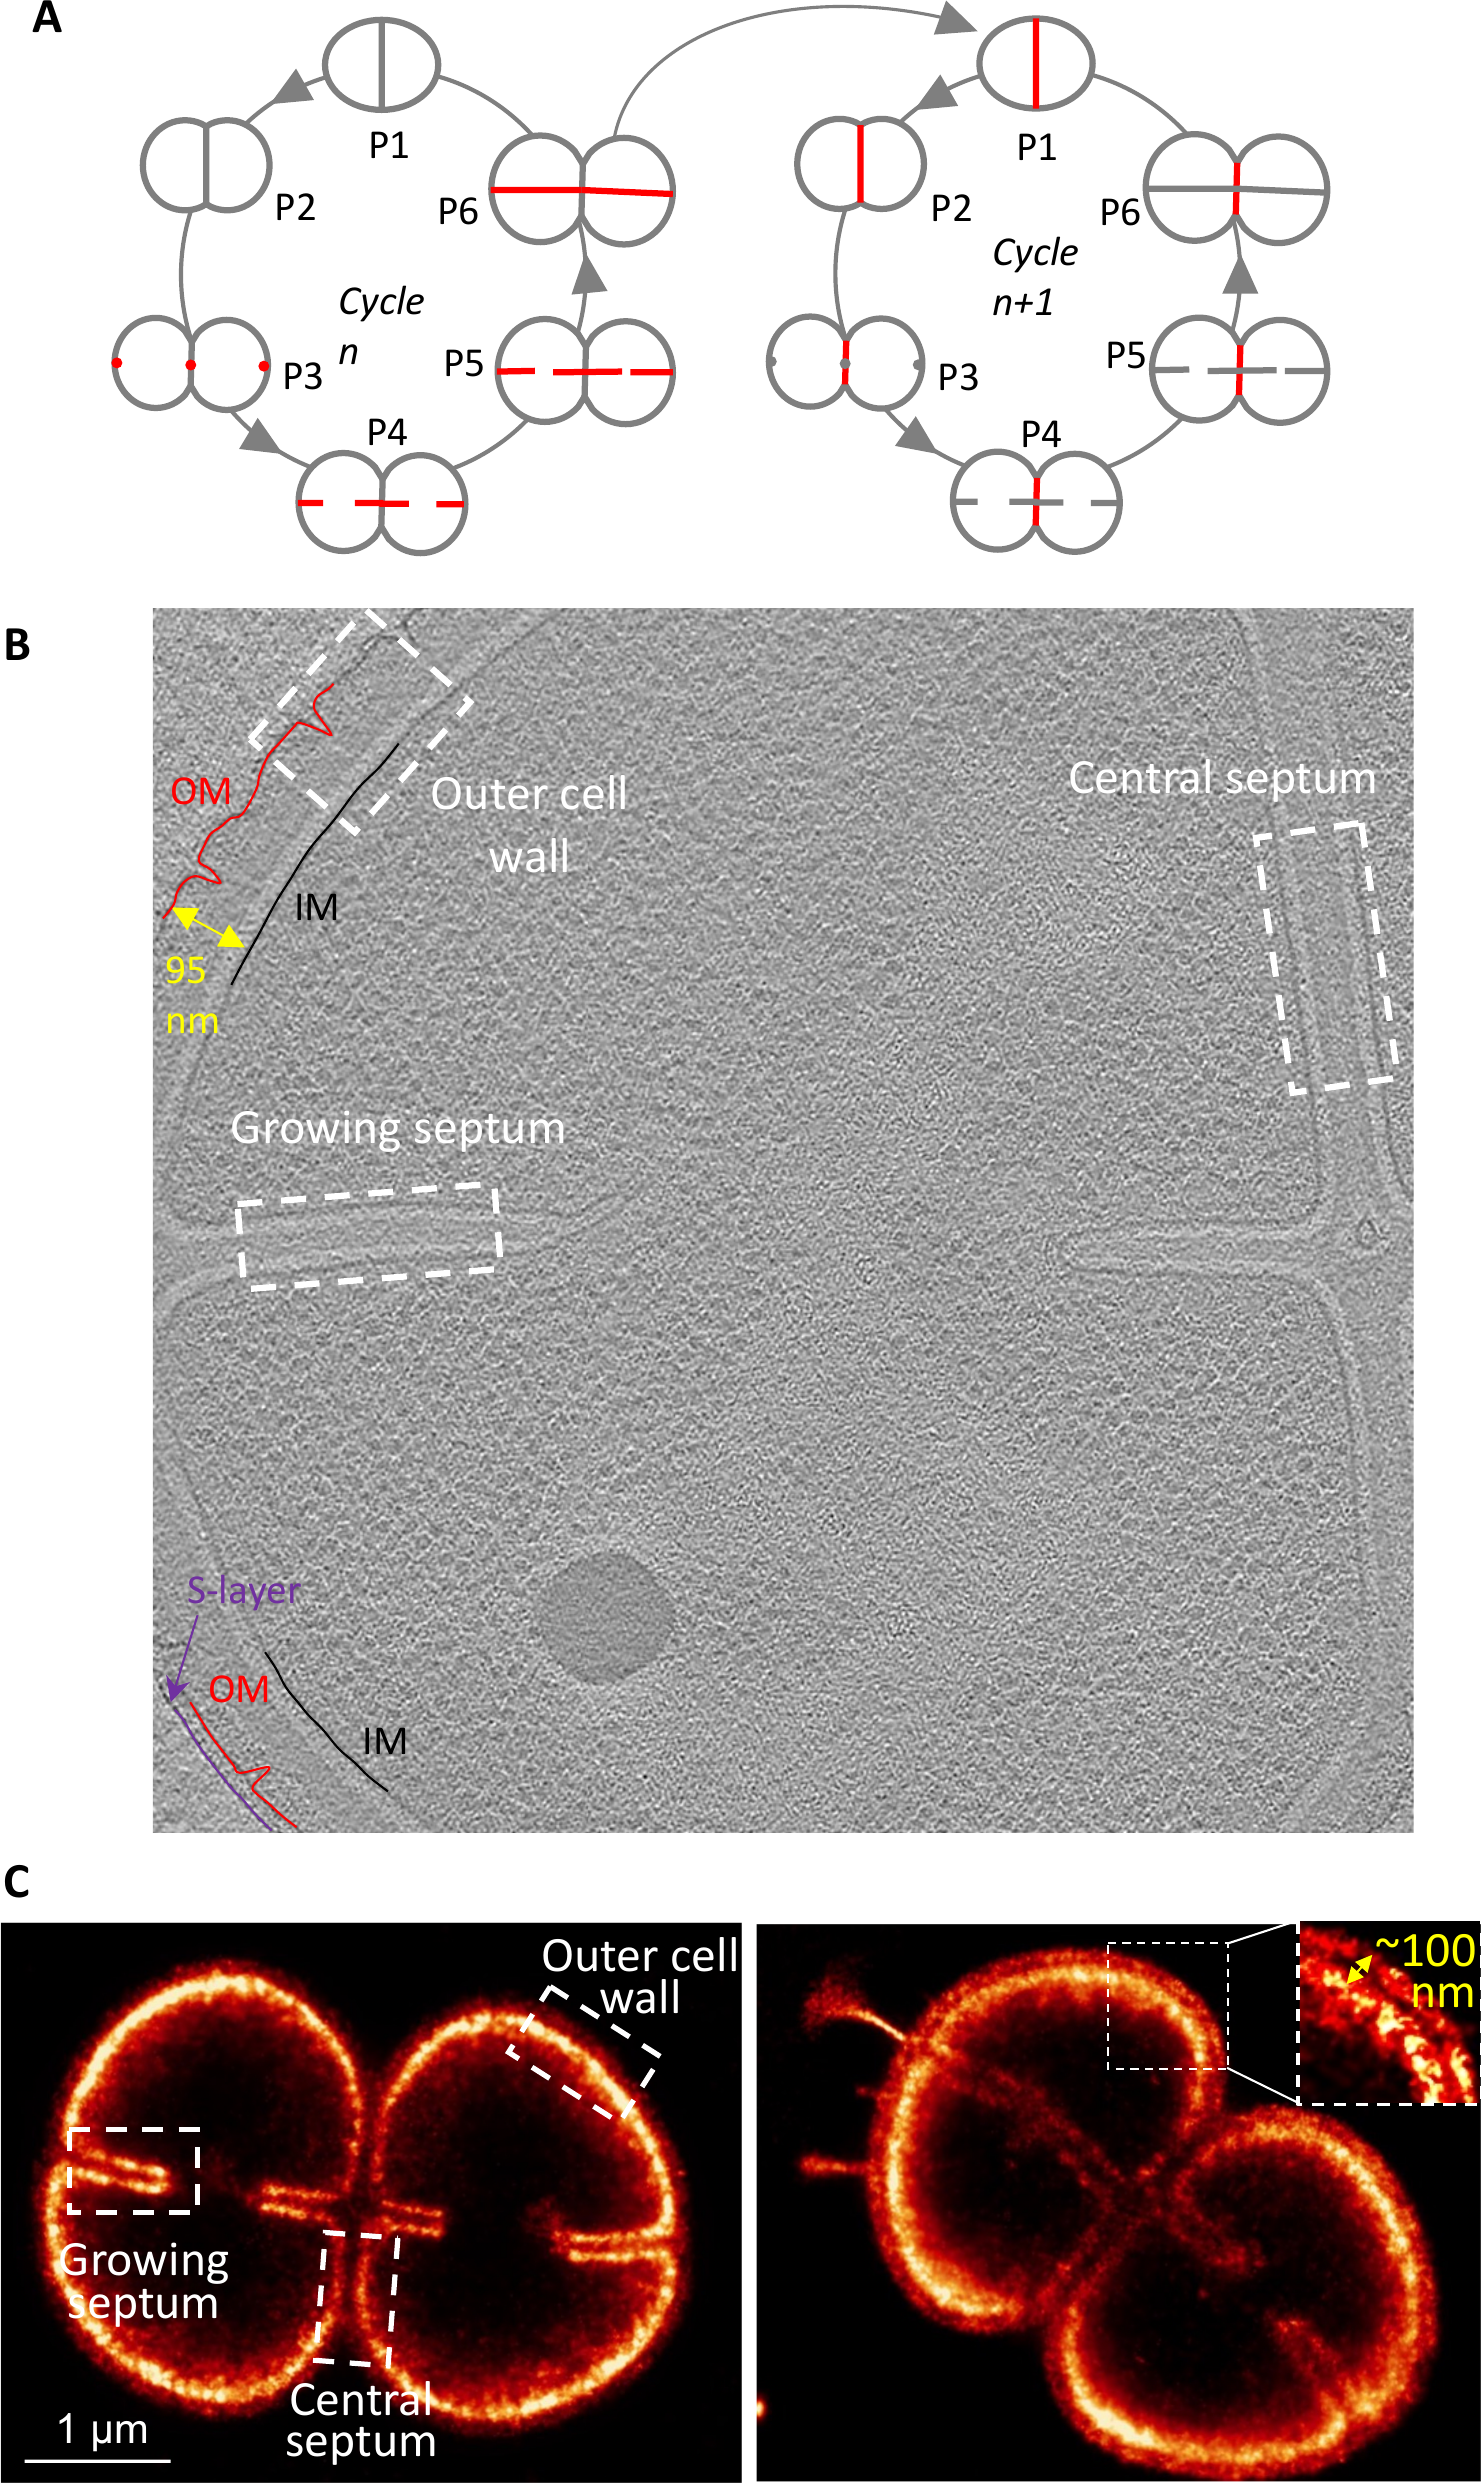
\includegraphics[width=.85\textwidth]{drad_paper/fig1.png}
    \titledcaption[Structures of exponentially growing D. radiodurans cell walls during the process of cell division]{(A) Averaged central slices through of a typical cryo-electron tomogram of an actively dividing wild-type D. radiodurans diad. Three different types of cell wall can be seen in this image: (i) the multilayered outer cell wall composed notably of both an inner (IM) and an outer (OM) membrane highlighted respectively in black and red, (ii) the central septum dividing the two cells composing the diad unit, and (iii) the new growing septa originating from opposite sides of the cell. The mean distance between the two membranes in the outer cell envelope was determined to be 95 nm. The light grey density in the center of the cell corresponds to the nucleoid and the darker densities in the cytoplasm are the ribosomes. Scale bar: 100 nm. (B) Two examples of super-resolved PAINT images of Nile Red stained wild-type D. radiodurans diads in the process of dividing. Nile Red specifically stains the plasma membrane. As in (A), three distinct regions of cell wall can be distinguished. On a few occasions, the two lipid bilayers of the outer cell envelope could be resolved (as in the right image). The mean distance between these two layers was determined to be 100 nm in good agreement with the 95 nm measured on the tomograms. Scale bar: 1 \mu{}m.}
    \label{drad_fig1}
\end{figure}

The outer cell wall bears two lipid bilayers that can be seen as dark lines in the cryo-ET data and could be distinguished on a few occasions in our super-resolved PAINT images of Nile Red stained \textit{D. radiodurans} (\autoref{drad_fig1}B, right panel).
The distance between the inner (IM) and outer (OM) cell membranes was in good agreement between the two techniques and was found to be around \qty{95}{nm} (\autoref{drad_fig1}).
A more in-depth analysis of the cell wall layer composition was facilitated by the preparation of straightened cell wall projections of the cryo-ET images using a recently developed tool, blik~\cite{gaifasBlikExtensible3D2024}.
Density profiles of the outer cell wall revealed that this region is composed of 6 distinct layers: (i) the IM, (ii) a low-density periplasmic space, (iii) a high-density PG layer, (iv) an intermediate layer previously described as the SlpA layer~\cite{vonkugelgenMultidomainConnectorLinks2022}, (v) the OM and (vi) a discontinuous hexagonally packed S-layer on the outer surface of the bacteria (\autoref{drad_fig2}A).
A distinctive white line was seen to separate the PG layer from the SlpA layer and V-shaped invaginations of the OM were seen regularly along this outer cell wall.
Measurements made on numerous cryo-ET datasets allowed us to determine the mean thickness of each of these 6 layers.
When present, the S-layer was typically located at \qty{18}{nm} above the OM, the SlpA layer was found to be \sim\qty{34.5}{nm} in thickness in good agreement with the estimated dimensions of the SlpA complex that stretches across this layer~\cite{vonkugelgenMultidomainConnectorLinks2022}.
The PG layer was found to be \sim\qty{42.5}{nm} in thickness and located approximately \qty{15}{nm} above the IM with a low-density region located in between these two essential layers.
Interestingly, these measurements revealed that the IM bilayer was significantly thicker than the OM (\qty{5.5}{nm} vs \qty{4.0}{nm}) suggesting distinct lipid compositions.

\begin{figure}[ht]
    \centering
    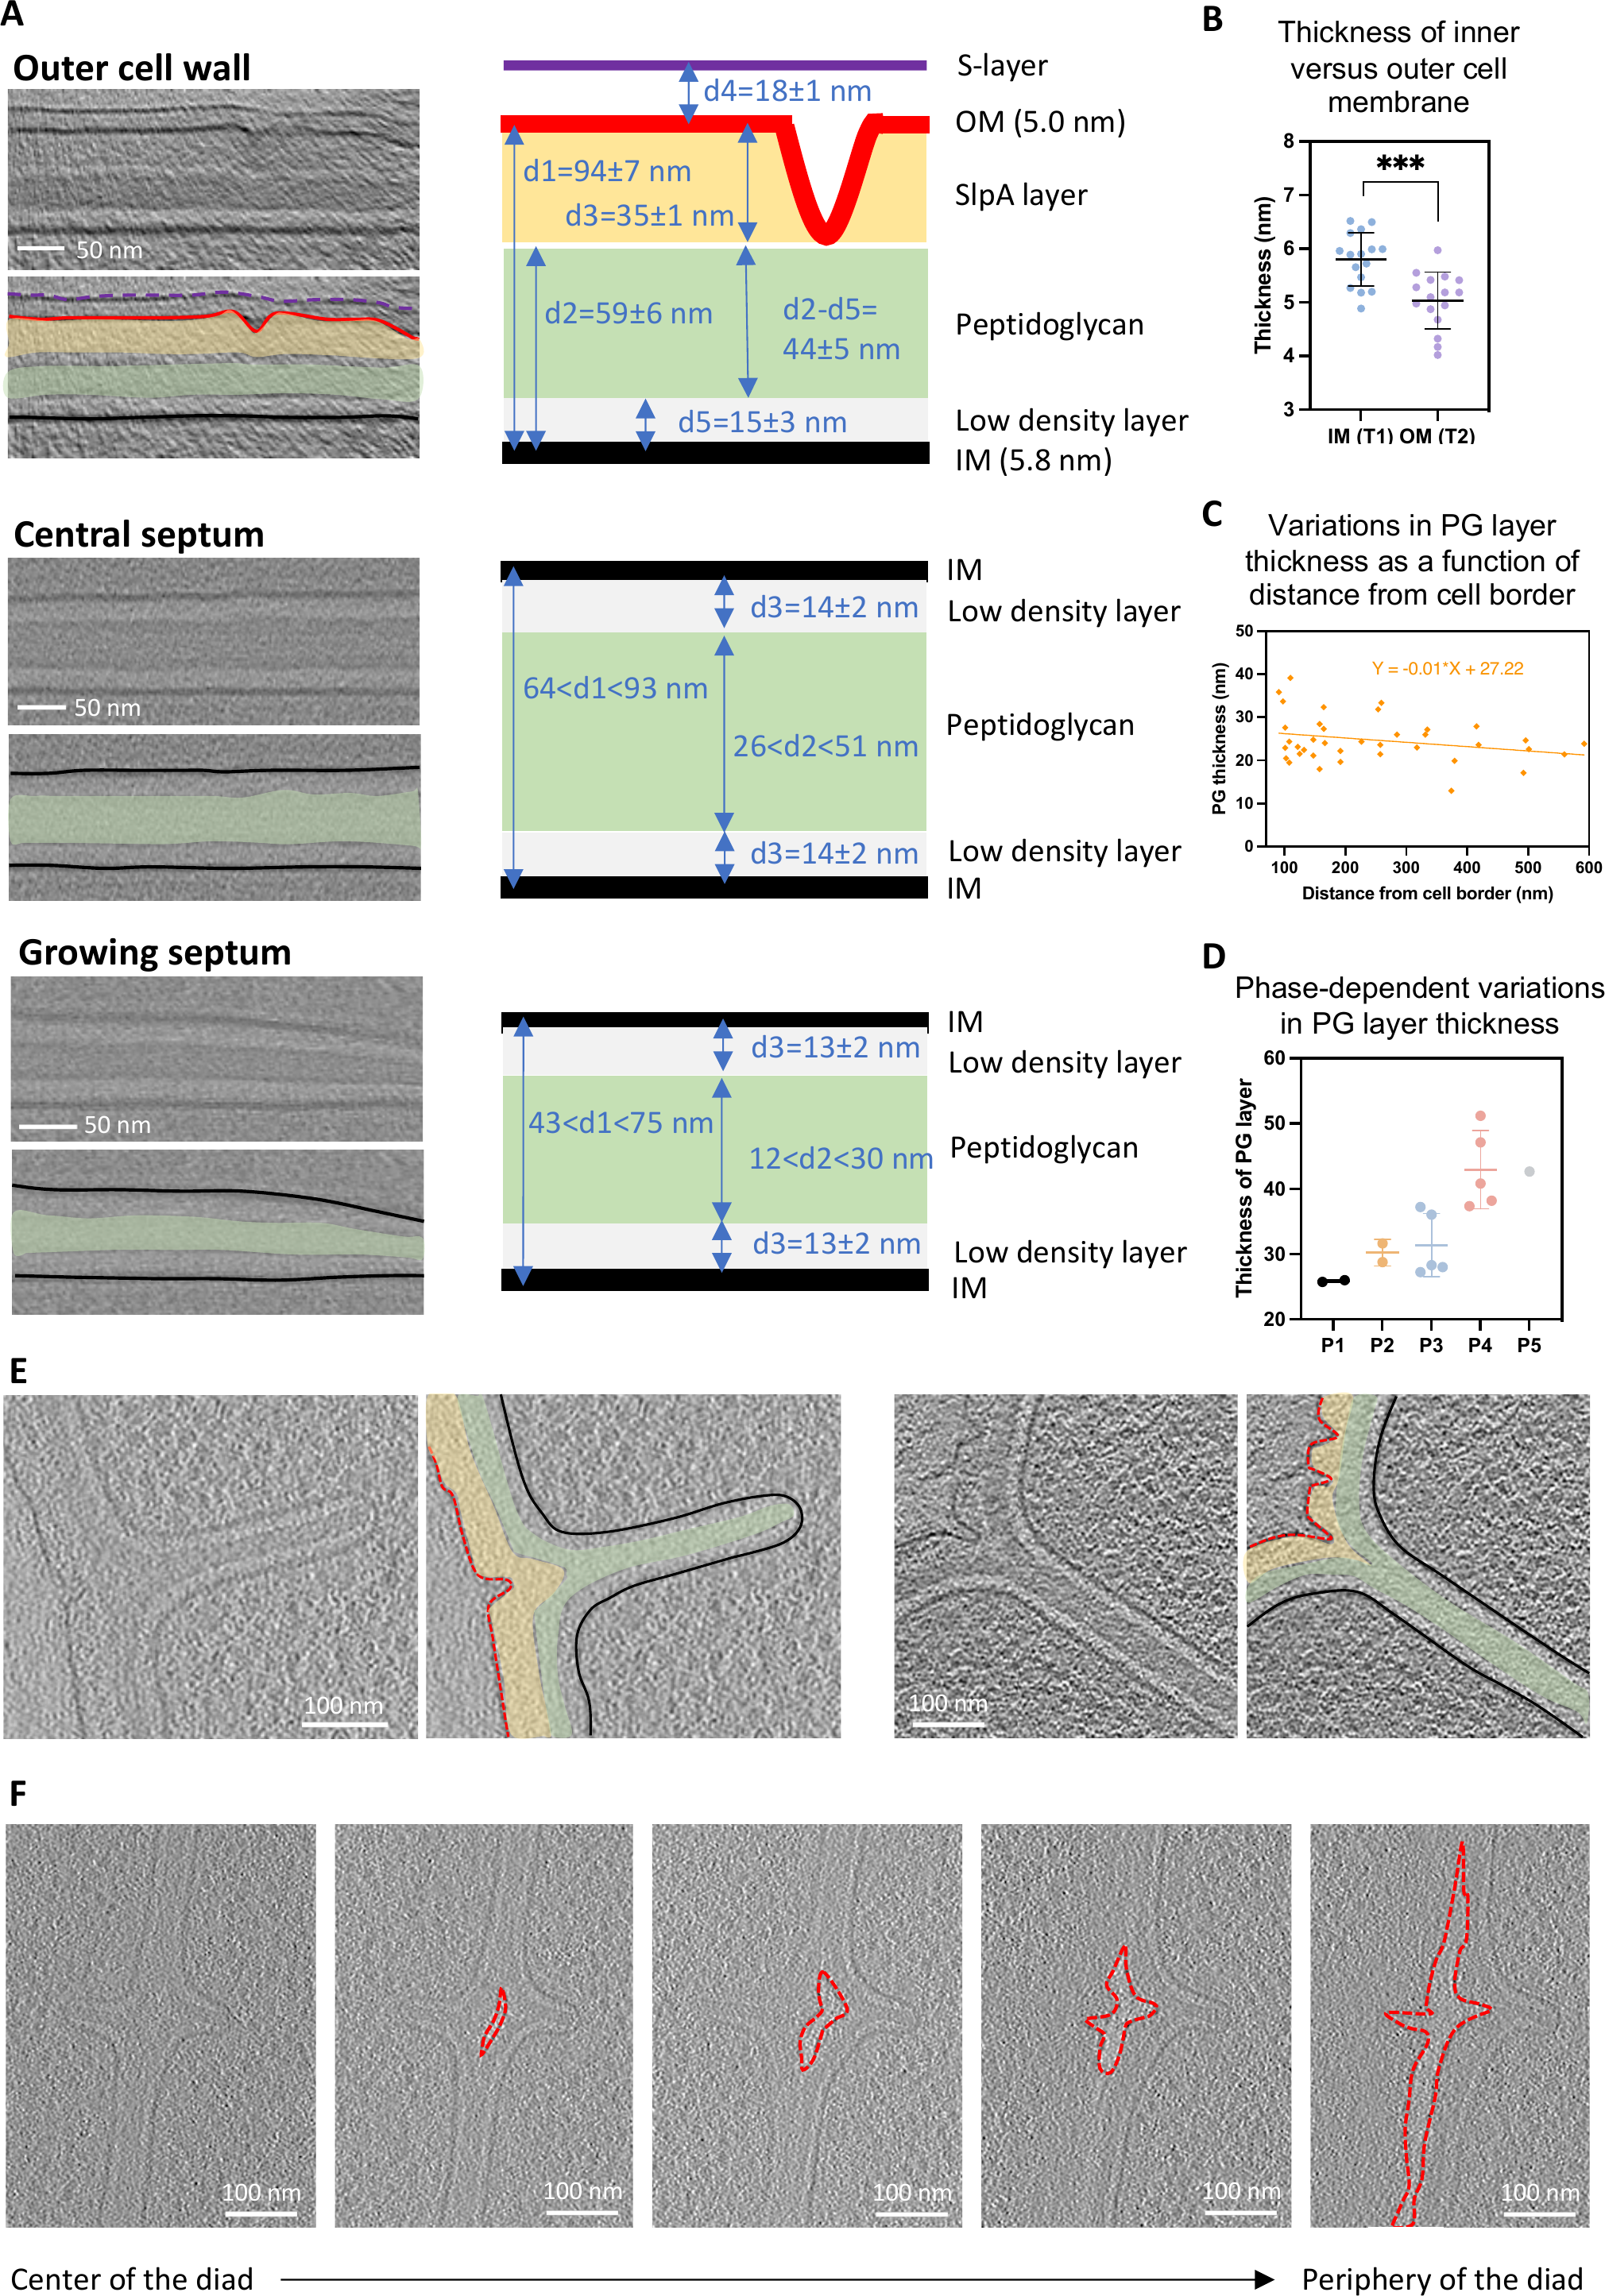
\includegraphics[width=.9\textwidth]{drad_paper/fig2.png}
    \titledcaption[In-depth analysis of the structure and composition of the cell wall of D. radiodurans]{(caption on the next page)}
    \label{drad_fig2}
\end{figure}
\begin{figure}[ht]
    \ContinuedFloat
    \caption[]{(A) Straightened sections of the outer (Top), central (middle) and growing septum (bottom) cell walls were used to measure the thickness of the various layers composing these three types of cell wall shown schematically to the right of the images (\autoref{drad_sfig8}) for more details). Left: Top panels show an averaged 2D slice an averaged and straightened 2D slice and lower panels show the same section with segmentations of the various layers. The IM is highlighted in black, the OM in red, the S-layer in purple, the SlpA layer in yellow, the peptidoglycan in green and the low-density periplasmic space in light grey. Scale bars: 50 nm. (B) Mean and standard deviation of the thickness of the inner (IM) and outer (OM) membranes within the outer cell envelope. N=16. Statistical test: Welch's t-test. *** p=0.0002. (C) Plot illustrating the phase-dependent thickness of the peptidoglycan (PG) layer in the central septum (d2 in \autoref{drad_sfig8}). Bars correspond to mean and standard deviation per phase (N<6 for each phase). Individual points correspond to the mean thickness measured on each tomogram. (D) Plot illustrating the variation in PG thickness as a function of the distance from the lagging edge of the growing septa. The PG layer was thinner at the leading edge than at the lagging edge of the growing septa. (E) Two illustrations of junctions between the outer cell envelope and the growing septa. Left panels show an averaged 2D slice through of a tomogram and right panels show the same regions with segmentations of the various layers (colors as in A). Scale bar: 100 nm. (F) Averaged 2D slices extracted from a given tomogram at different z values illustrating the progressive splitting of daughter cells that starts at the cell periphery (right) and then progresses inwards towards the center of the diad (left). The progressive synthesis of the outer lipid bilayer is shown in red. Scale bar: 100 nm.}
\end{figure}

A similar procedure was used to analyse the composition of the growing septa and the central cell wall region.
The outer layers of the external cell wall (S-layer, OM and SlpA layer) were missing in these regions (\autoref{drad_fig2}A), and instead septa were composed of a single central continuous PG layer with the IM and the low-density periplasmic space on either side.
These three layers were continuous with those of the outer cell envelope.
While the IM bilayer and low-density periplasmic space showed similar thicknesses in these two locations, the PG layer displayed significant variations, ranging from \qty{42}{nm} to \qty{56}{nm} in the central cell wall and as low as \qty{35}{nm} in the growing septa.
In both the growing septa and the central cell wall, the PG layer was typically thicker at the cell periphery than at the leading edge of the septum or the centre of the diad respectively, and in the central cell wall, the mean thickness of the PG layer was also found to vary substantially as a function of the phase of the cell cycle, suggesting a progressive thickening of this layer until reaching its final size prior to the splitting of the diad (\autoref{drad_fig2}A).

At the junction between the outer cell wall and the lagging edge of the growing septum (\autoref{drad_fig2}B and \autoref{drad_sfig2} for more examples), we observed that the PG and low-density periplasmic layers followed the IM, while the outer layers (SlpA layer and OM) were restricted to the outer cell wall.
V-shaped invaginations in the OM were often observed at these junctions and were found to extend inwards during the splitting of the two daughter cells during the subsequent cell cycle.
As shown in \autoref{drad_fig2}C, cell splitting is a progressive process, most likely initiated from the cell periphery and moving inwards from both the top and the bottom of the cell towards the center of the diad forming bubble-like membrane structures (\autoref{drad_sfig1}B for more examples).
Splitting occurs concomitantly with the addition of the SlpA layer and finally the OM to the central septum cell wall (\autoref{drad_fig2}C).

\FloatBarrier

\subsection{Structure of septal tips}

A close inspection of the tomograms revealed that the tips of the growing septa exhibited particular structures.
A majority of septa (40 of the 64 septa visible in our tomograms) were slightly tapered at their tips and the low-density periplasmic space was significantly thinner in these regions bringing the PG layer very close to (in some cases even touching) the IM (\autoref{drad_fig3}A).
Strikingly, in nearly 40\% of the observed septa, membrane protrusions, reported in earlier studies as mesosomes~\cite{thornleyFineStructureMicrococcus1965,sleytrStudyFreezeetchingFine1973}, were observed at the tips of growing septa (\autoref{drad_fig3}B-C and \autoref{drad_sfig2} for more examples).
These structures appear to be composed solely of the low-density layer and are delimited by the IM bilayer.
They were mostly observed in cells in early stages of the septation process bearing short septa.
In 2D micrographs, these extensions adopt either extended tube-like structures or more circular loop-like arrangements.
In all cases, they appear to be very flexible, probably as a result of the absence of a PG layer to rigidify the protrusion.
This intrinsic flexibility may explain why the tips of the growing septa were often not observed in the super-resolved images of Nile Red-labelled \textit{D. radiodurans} cells (\autoref{drad_fig3}C, left panel).
Instead, in these images, open ends were observed at the leading edge of the growing septa.
This suggests that either the Nile Red dye poorly labelled these highly curved membrane bilayers likely exhibiting reduced membrane fluidity that is known to affect Nile Red staining~\cite{strahlActinHomologueMreB2014} or that the tips were very mobile and not captured in live imaging experiments.
Both of these phenomena may also be at play.
On a few occasions, we did nonetheless observe poorly defined Nile Red labelling at the tips of growing septa that may correspond to these flexible membrane protrusions (\autoref{drad_fig3}C, right panel).

\begin{figure}[ht]
    \centering
    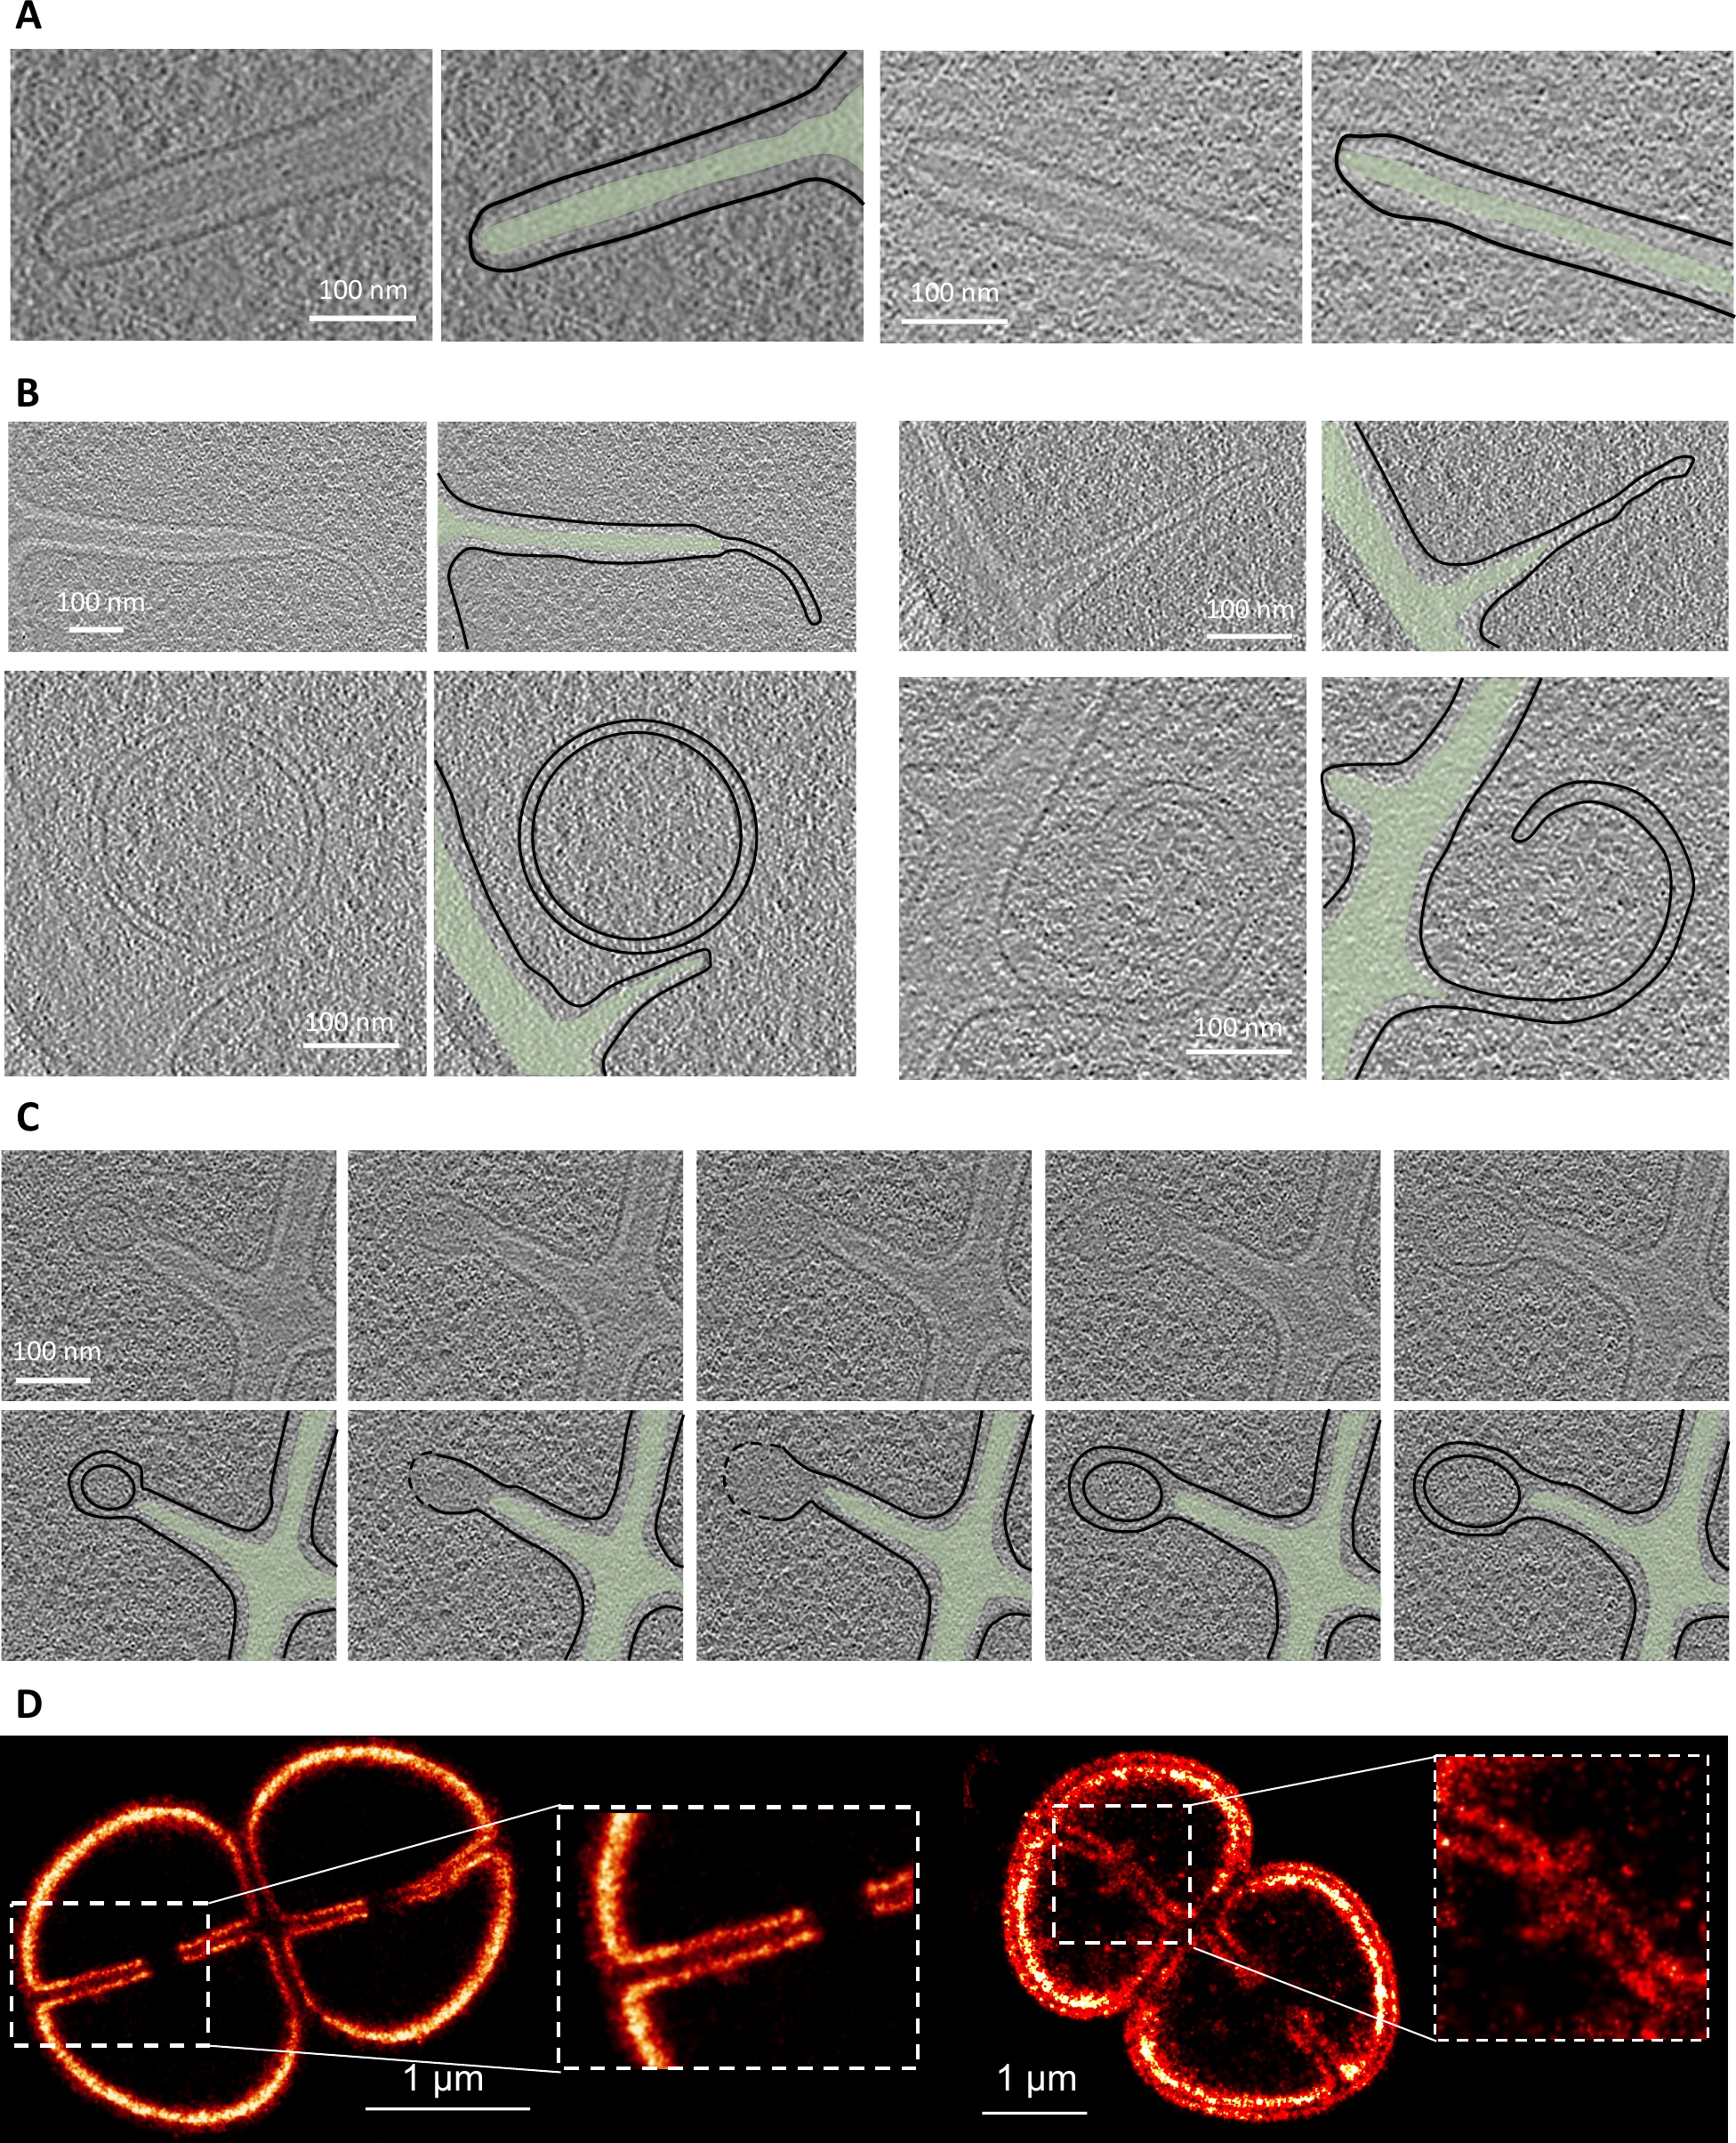
\includegraphics[width=\textwidth]{drad_paper/fig3.png}
    \titledcaption[Close-up view of the septal tips]{(caption on the next page)}
    \label{drad_fig3}
\end{figure}
\begin{figure}[ht]
    \ContinuedFloat
    \caption[]{(A-B) Examples of typical septa tip morphologies: (A) tapered leading edge with a well-defined and rigid PG layer (green) stretching almost to the IM (black) and (B) tubular (top) and curved (bottom) membrane protrusions extending the growing septa. Left panels show an averaged 2D slice through of a tomogram and right panels show the same regions with segmentations of the various layers (colors as in Fig. 2A). (C) Averaged 2D slices extracted from a given tomogram at different z values illustrating the change in size and shape of these membrane protrusions as a function of the position in the tomogram. Top panels show averaged 2D slices and lower panels show the same regions with segmentations of the PG and IM layers (colors as in Fig. 2A). (A-C) Scale bar: 100 nm. (D) Close-up views of the leading edges of growing septa captured by super-resolution PAINT microscopy of Nile Red stained wild-type D. radiodurans diads in the process of dividing. Left image: septal tips appear to be open-ended with no obvious fluorescence signal for the highly curved membrane located at the leading edge of these closing septa. Right image: blurry septal tips are visible pointing in opposite directions. These structures may correspond to the membrane protrusions observed in the tomograms (B, C). Scale bar: 1 \mu{}m.}
\end{figure}

\FloatBarrier

\subsection{Septation through a "sliding door" mechanism}

Using timelapse 3D video confocal microscopy of Nile Red stained \textit{D. radiodurans} bacteria immobilized in various orientations on agarose pads (\autoref{drad_sfig3}B), we followed the division process in live cells.
Septation was found to involve several steps.
First, two septa originating from opposite sides of the cell grow inwards with a flat leading edge creating a central gap stretching from the top to the bottom of the cell.
As the septa grow, the leading edge progressively becomes more curved forming a cat's eye structure in between the two opposite septa.
Finally, when the two septa come close to each other, fusion starts first at the top and bottom of the cell and then rapidly proceeds through a zipping mechanism from the cell periphery to the cell center.
3D super-resolved (PAINT) images of Nile Red labelled \textit{D. radiodurans} cells confirmed these observations, allowing to capture high-resolution snapshots of dividing cells exhibiting septa with flat or slightly curved leading edges embracing a central gap that stretches all across the cell (\autoref{drad_fig4}A).
Kymographs of individual septation events were extracted from the live cell confocal acquisitions to probe the kinetics of this process (\autoref{drad_fig4}B).
These revealed that septation is a linear process in which the external and internal septa grow respectively at rates of \qty{7.3(0.5)}{nm.min^{-1}}  and \qty{4.1(0.7)}{nm.min^{-1}} until full closure.
Interestingly, the external septum starts growing ahead of the internal septum, as can be seen from the asymmetric V-shaped structure of the kymographs, and grows at a faster rate than the internal septum (\autoref{drad_fig4}B).
This may be explained by the fact that the external septum needs to grow further than the internal septum to reach the site of fusion located at mid-cell and has to compensate for the expansion of the cells that is occurring simultaneously (\autoref{drad_fig4}A).
A flat leading edge and an asymmetric growth of the external and internal septa were also observed in our cryo-ET data, which captured bacteria at various stages of the division process (\autoref{drad_fig4}C-D).

\begin{figure}[ht]
    \centering
    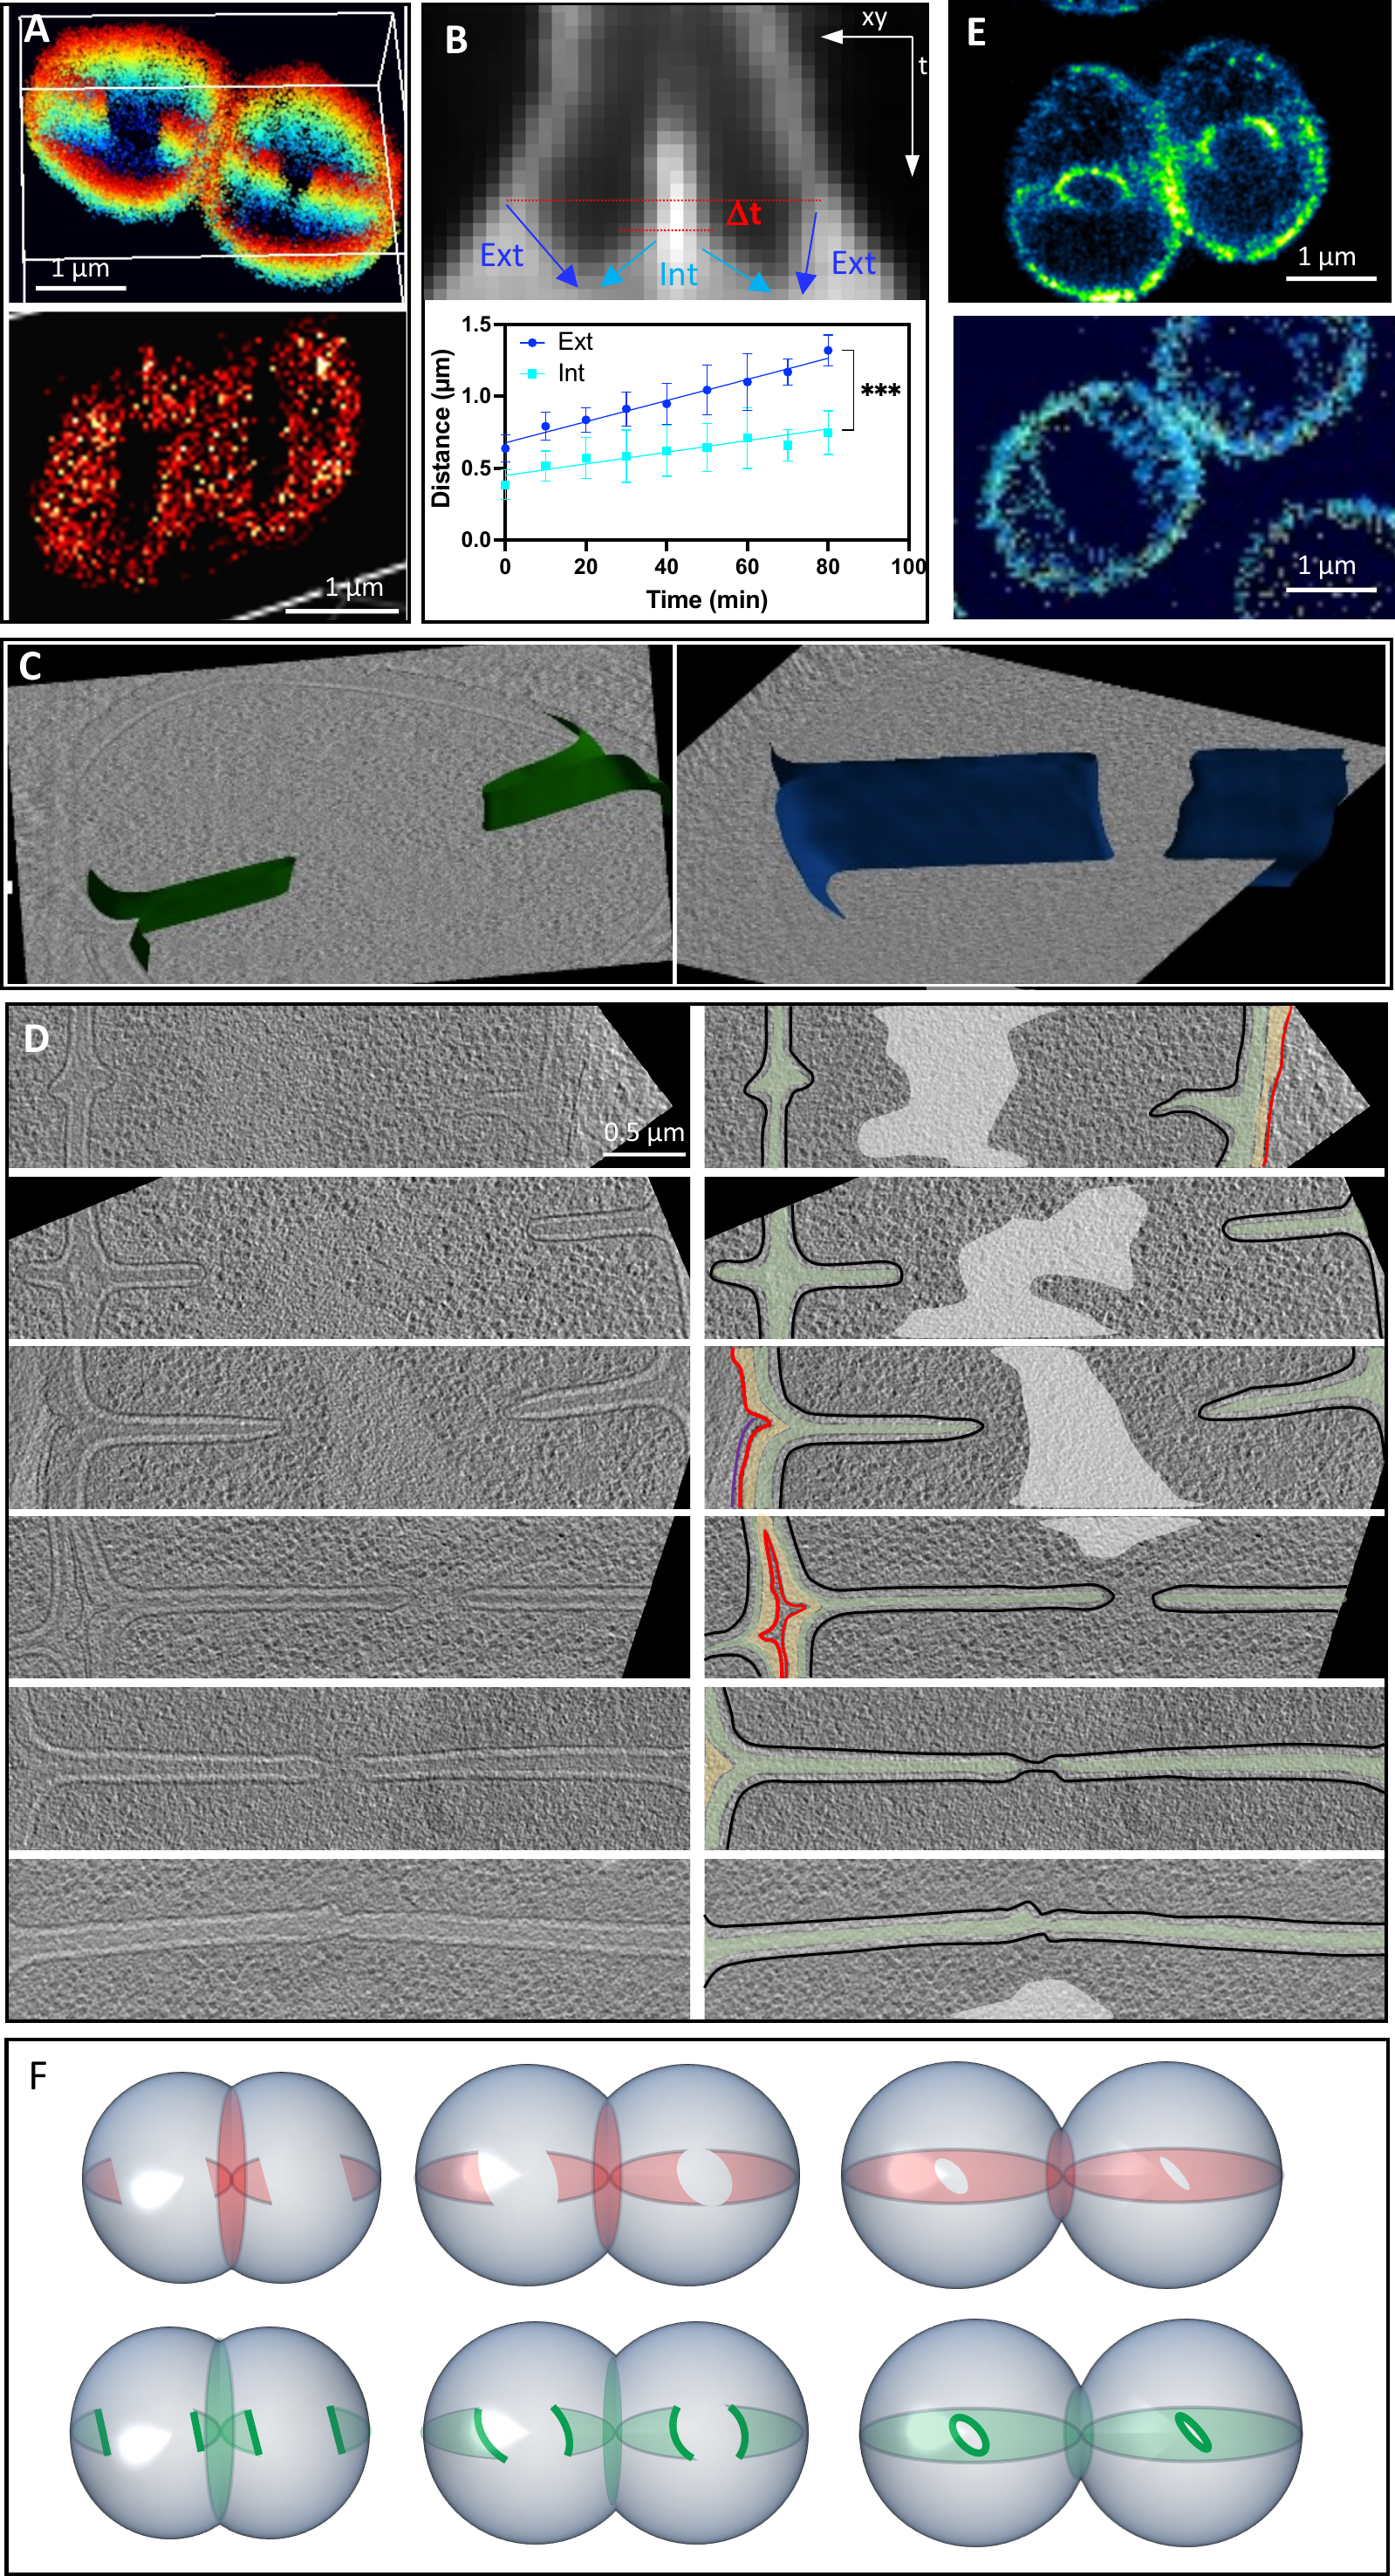
\includegraphics[width=.75\textwidth]{drad_paper/fig4.png}
    \titledcaption[Septation through a "sliding door" mechanism]{(caption on the next page)}
    \label{drad_fig4}
\end{figure}
\begin{figure}[ht]
    \ContinuedFloat
    \caption[]{(A) 3D super-resolved PAINT image of a Nile Red stained wild-type D. radiodurans diads in the process of dividing. Top panel: the 3D volume was obtained by combining XXX stacks of images collected at different focus heights. The flat leading edge is very clear in the left cell while the right cell, which is more advanced in its division process, illustrates the formation of a cat's eye structure stretching across the cell as the opposing septa first meet and fuse at the top and bottom of the cells. This structure is also visible in the lower panel, corresponding to a Z-slice through a labelled cell. Scale bar: 1 \mu{}m. (B) Kymograph analysis of the septation process in Nile Red stained D. radiodurans. Top panel: example of a typical kymograph obtained for a dividing diad. The coordinates of the borders of the fluorescent signal were used to determine the length of the external (dark blue) and internal (light blue) septa as a function of time. The lag time (Dt) between the start of septal growth for the external septa versus the internal septa was also measured. Lower panel: Plot illustrating the linear growth of the external (dark blue) and internal (light blue) septa as a function of time. The external septa were found to grow at a significantly higher rate than the internal septa. *** (p-value: 0.0004). (C) Examples of segmented septa in two tomograms illustrating the flat edge of the growing septa (left panel, green) that progressively becomes more curved (right panel, blue) as the division process advances. (D) Averaged 2D slices extracted from various tomograms illustrating different stages of the septation process in D. radiodurans. Left panels show an averaged 2D slice through of a tomogram and right panels show the same regions with segmentations of the various layers (colors as in Fig. 2A). The light grey annotation in the panels on the right corresponds to the nucleoid. Scale bar: 0.5\mu{}m. (E) 3D super-resolved dSTORM image of PG-labelled (through incorporation of azido-D-Alanine) wild-type D. radiodurans diads in the process of dividing. Top panel: PG synthesis occurs both in the septa and in the outer cell wall with a strong PG synthesis activity detected at the leading edge of the growing septa (intense ring and arch). Lower panel: Z-slice through a PG-labelled D. radiodurans diad illustrating the incorporation throughout the septal region and the formation of the cat's eye structure similar to that observed in Nile Red stained cells (A). Scale bar: 1 \mu{}m. (F) Schematic model of the "sliding door" mechanism of septation in D. radiodurans. The top panels illustrate the Nile Red labelled membrane growth (red), while the lower panels show the closely-related growth of the PG layer and the strong PG synthesis activity at the leading edge of the septa.}
\end{figure}
% TODO: fill in the XXX above

In addition to staining the cell membrane, we also labelled the PG layer of \textit{D. radiodurans} cell walls by incorporating modified azido-D-alanine (aDA) into the cell wall that was subsequently labelled by copper free click chemistry with fluorescent probes suitable for either confocal or dSTORM microscopy~\cite{trouveNanoscaleDynamicsPeptidoglycan2021,trouveMetabolicBiorthogonalLabeling2021} (\autoref{drad_sfig4}).
The PG labelling pattern (\autoref{drad_fig4}E and \autoref{drad_sfig5}) was very similar to that of Nile Red labelled cells, with an efficient incorporation occurring in all regions of the cell wall (septal, central and outer cell walls) as was observed previously using fluorescently labelled D-alanine~\cite{flochCellMorphologyNucleoid2019}.
The main difference was that the PG labelling was more prominent at the leading edge of the growing septa than elsewhere, suggesting this likely corresponds to the major site of active PG synthesis in these dividing cells (\autoref{drad_fig4}F).
This is particularly visible at late stages of the cell cycle, either just before (Phase 5) or just after cytokinesis (Phase 6), where an intense band of labelled PG can be seen at the site of fusion where the two opposing septa meet (\autoref{drad_sfig5}C).
In agreement with these observations, pulse-chase experiments in which bacteria were returned to the incubator for 45 minutes (chase) after incorporation of the modified aDA (pulse) into their cell walls, revealed that septa having incorporated aDA labelling at their tips during the pulse period, were progressively extended further by unlabelled PG, indicating that new PG is added to the existing layer in an inwards direction until the opposing septa are close enough to fuse (\autoref{drad_fig4}F and \autoref{drad_sfig6}).

Close examination of the tomograms also revealed that the position and shape of the growing septa changed as a function of their length (\autoref{drad_fig4}D).
At early stages of the septation process, short septa were not always precisely facing each other and their tips were often bent and bearing membrane protrusions, while at later stages, septa were remarkably straight and fully aligned to ensure fusion of the septa originating from opposite sides of the cell.
The presence of a PG layer in the growing septa appears to be a pre-requisite for the formation of these straight and well-aligned septa, indicating that the synthesis of the PG layer may provide the necessary rigidity to the growing cell walls for the final closure.
This final fusion step was captured in two of the tomograms and was found to proceed first through fusion of the IM bilayers and subsequently through synthesis of PG to fill the gap and "\textit{glue}" the two septa together (\autoref{drad_fig4}S).
Taken together, these data allow us to propose a model for septation through the "sliding doors" mechanism, which is illustrated schematically in \autoref{drad_fig4}F.

\FloatBarrier

\subsection{PG synthesis in the outer cell wall and in the septa are performed by distinct machineries}

To better understand the molecular mechanisms underlying this unusual mode of septation, we treated \textit{D. radiodurans} cultures with the \beta-lactam antibiotic, ampicillin, and compared the growth of untreated and treated Nile Red labelled cells by 3D confocal timelapse microscopy for a three-hour period.
Ampicillin is known to bind to the active sites of certain PBPs, thereby inhibiting their enzymatic cell wall synthesis function~\cite{sauvageGlycosyltransferasesTranspeptidasesPenicillinBinding2016}.
To our surprise, septation but not cell growth was arrested by ampicillin treatment (\autoref{drad_fig5}).
Indeed, the growth of the outer cell perimeter was unaffected by this treatment during this three-hour period, while growth of both the internal and external septa were rapidly arrested (\autoref{drad_fig5}B-C).
After 1 hour, the septa even started to shorten, suggesting they may be undergoing disassembly and degradation (\autoref{drad_fig5}C).
As a result of this change in the balance between cell growth and septation, cells progressively became distorted (more elongated with a slight bulge at sites of division) as evidenced by the substantially increased diameter (d) to perimeter (p) ratio after three hours of treatment with ampicillin (\autoref{drad_fig5}D).
The specific inhibition of septal growth by ampicillin suggests that the PBPs responsible for PG synthesis and maturation in the septa are distinct from those involved in outer cell wall growth.

\begin{figure}[ht]
    \centering
    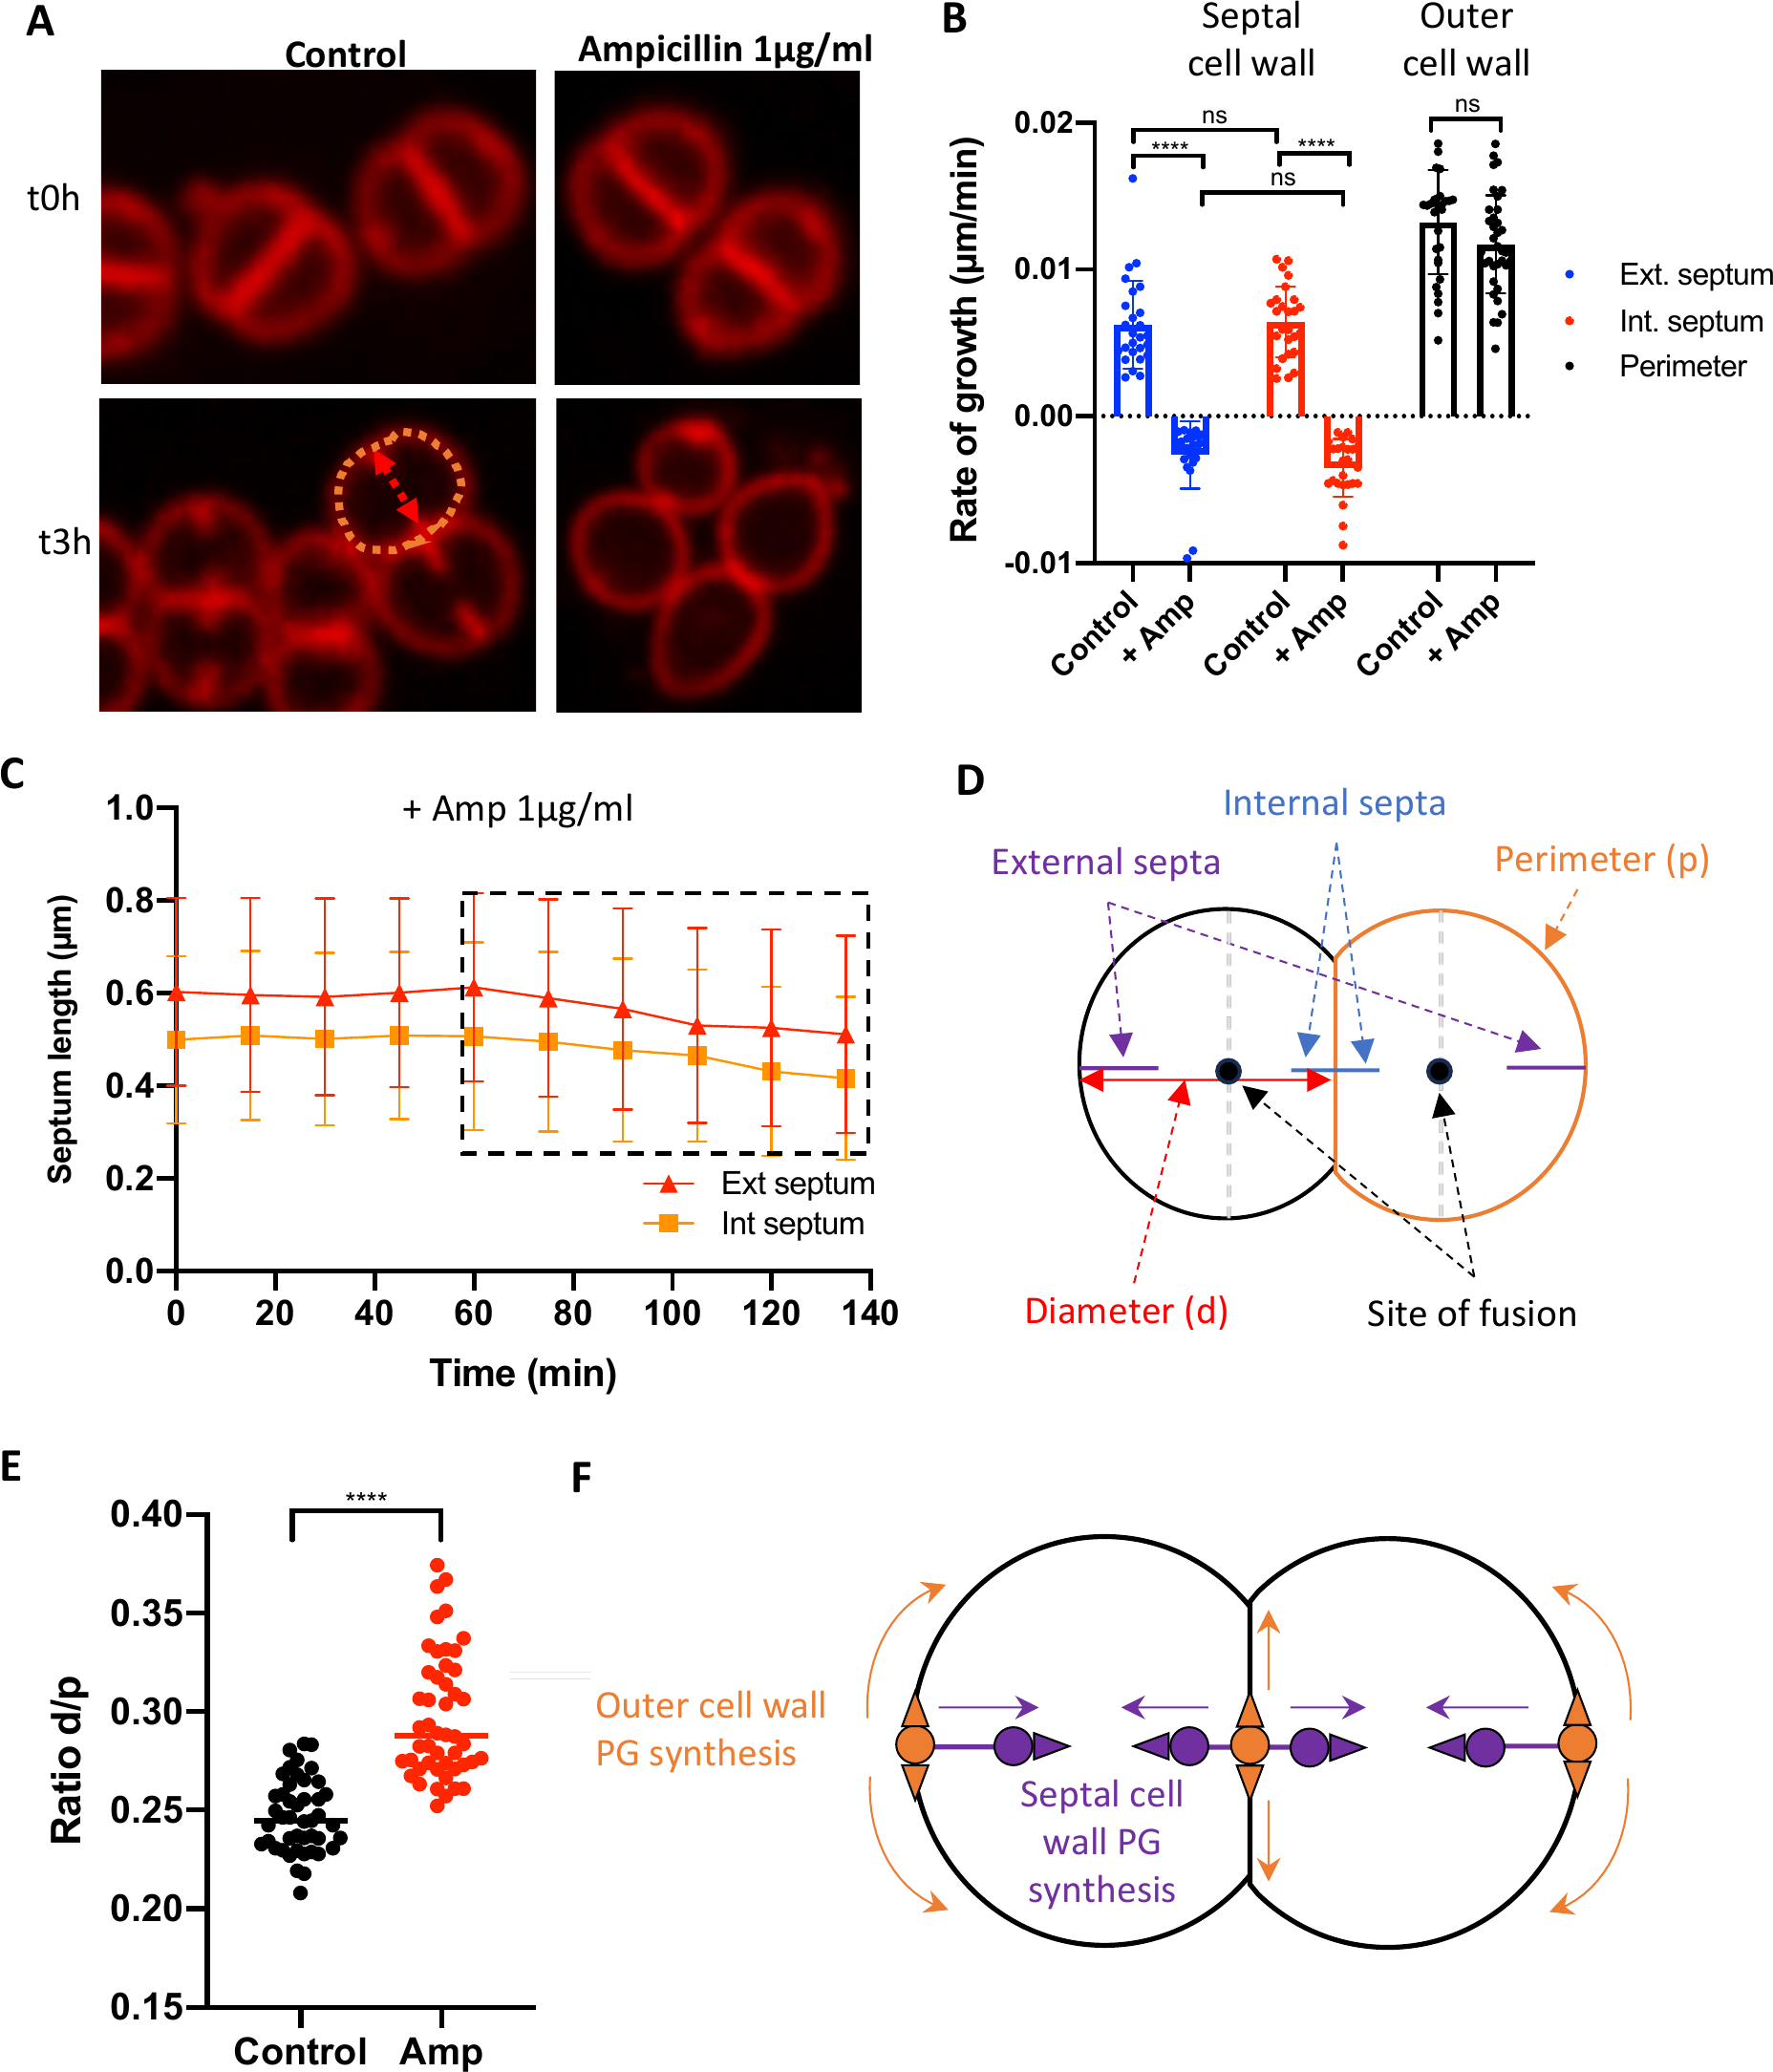
\includegraphics[width=.9\textwidth]{drad_paper/fig5.png}
    \titledcaption[Distinct PG synthesis machineries are involved in septal and outer cell wall growth]{(caption on the next page)}
    \label{drad_fig5}
\end{figure}
\begin{figure}[ht]
    \ContinuedFloat
    \caption[]{(A) Schematic diagram of a D. radiodurans diad, illustrating the different features and measurements made to probe the effect of ampicillin treatment. (B) Effects of ampicillin treatment on the growth rate of the external (blue) and internal (red) septa, and of the outer cell wall (black) corresponding to the perimeter of the cells. N>25. Statistical test: One-way ANOVA. Ns: non-significant, **** p-value < 0.0001. (C) Plot illustrating the inhibition of both the external (red) and internal (orange) septal growth by treatment with 1\mu{}g/ml ampicillin. After 1h of treatment, the lengths are the septa shorten suggesting they are being degraded. (D) Examples of untreated (left) and ampicillin-treated (right) Nile Red stained D. radiodurans at the start (t0h) and end (t3h) of the time-lapse experiment. Distortion of the cell morphology as a result of ampicillin treatment is particularly visible and is reflected in the marked change in the diameter:perimeter ratio (right) that is significantly increased in the presence of ampicillin (red). N>45. Statistical test: unpaired t-test. **** p-value < 0.0001. (E) Schematic model of the two PG synthesis machineries at play in D. radiodurans. The outer cell wall PG synthesis machinery (orange) appears to be insensitive to ampicillin and may well be localized to the junction between the outer cell envelope and the growing septa. In contrast, the septal PG synthesis machinery (purple) is very sensitive to ampicillin and is located mainly at the leading edge of the growing septa.}
\end{figure}

Next, we repeated the aDA incorporation experiment on cells pre-grown for either 1 or 2h in the presence of ampicillin before the labelling (\autoref{drad_sfig7}).
In these conditions, aDA was still readily incorporated into the outer cell wall, as expected based on our timelapse experiments.
In contrast, no labelling was seen in the septal regions, except at sites of septation initiation at the junction between the outer cell wall and the budding of the new septa, where a distinctive bright PG-labelled ring was observed (\autoref{drad_sfig7}).
These rings were occasionally seen in untreated cells, but were much more abundant in ampicillin-treated cells and in particular in samples pre-grown for 2 hours in the presence of the \beta-lactam antibiotic, where approximately 50\% of the cells displayed such ring-shaped PG labelling (\autoref{drad_sfig7}B).
The initial PG synthesis at the start of septation thus appears to be unaffected by ampicillin, while subsequent growth and extension of the septa is fully arrested by this treatment.
A shared PG machinery located at the junction between the outer cell wall and the start of septation may therefore be involved in both outer cell wall synthesis and initiation of septation, but a distinct set of proteins likely located at the leading edge of the growing septa appear to be responsible for PG synthesis across the dividing cells (\autoref{drad_fig5}E).
This finding is supported also by the pulse-chase experiments (\autoref{drad_sfig6}) in which we observed that most of the labelling of the septal regions, but not of the outer cell walls was lost after the chase period, indicating that the PG structure and/or maturation process are quite distinct in these two types of cell wall.

\FloatBarrier

\subsection{FtsZ is present at the tips of septa}\label{drad_ftsz}

We investigated the location of FtsZ, one of the key players in bacterial cell division, in dividing \textit{D. radiodurans} cells using both fluorescence microscopy and cryo-ET.
Two strategies were used to fluorescently label FtsZ: (i) immunolabelling of an endogenously HA-tagged FtsZ or (ii) endogenous tagging of FtsZ with a photoconvertible fluorescent protein, mEos4B.
The latter was compatible with live cell imaging, but this genetically modified strain of \textit{D. radiodurans} showed altered cell morphology (forming many large cells with likely impaired septation) and only a small fraction of cells exhibited fluorescence signal and visible Z-rings (\autoref{drad_fig6}A).
In contrast, the strain expressing HA-tagged FtsZ grew very well with no obvious morphological defects and FtsZ could be detected with an anti-HA antibody, after fixing and permeabilizing the cells, by either confocal or dSTORM microscopy (\autoref{drad_fig6}A-B).
Both strategies indicated that \textit{D. radiodurans} FtsZ forms ring- or oval-shaped structures of various sizes as reported for other bacteria, some of which appear to be incomplete.
Dual labelling of FtsZ and the cell membrane also revealed that FtsZ locates to the leading edge of growing septa at all stages of septation, including very early stages when septa are not yet visible by fluorescence microscopy (\autoref{drad_fig6}B).
At these early stages, FtsZ also appeared to form mostly incomplete Z-rings (\autoref{drad_fig6}B).

\begin{figure}[ht]
    \centering
    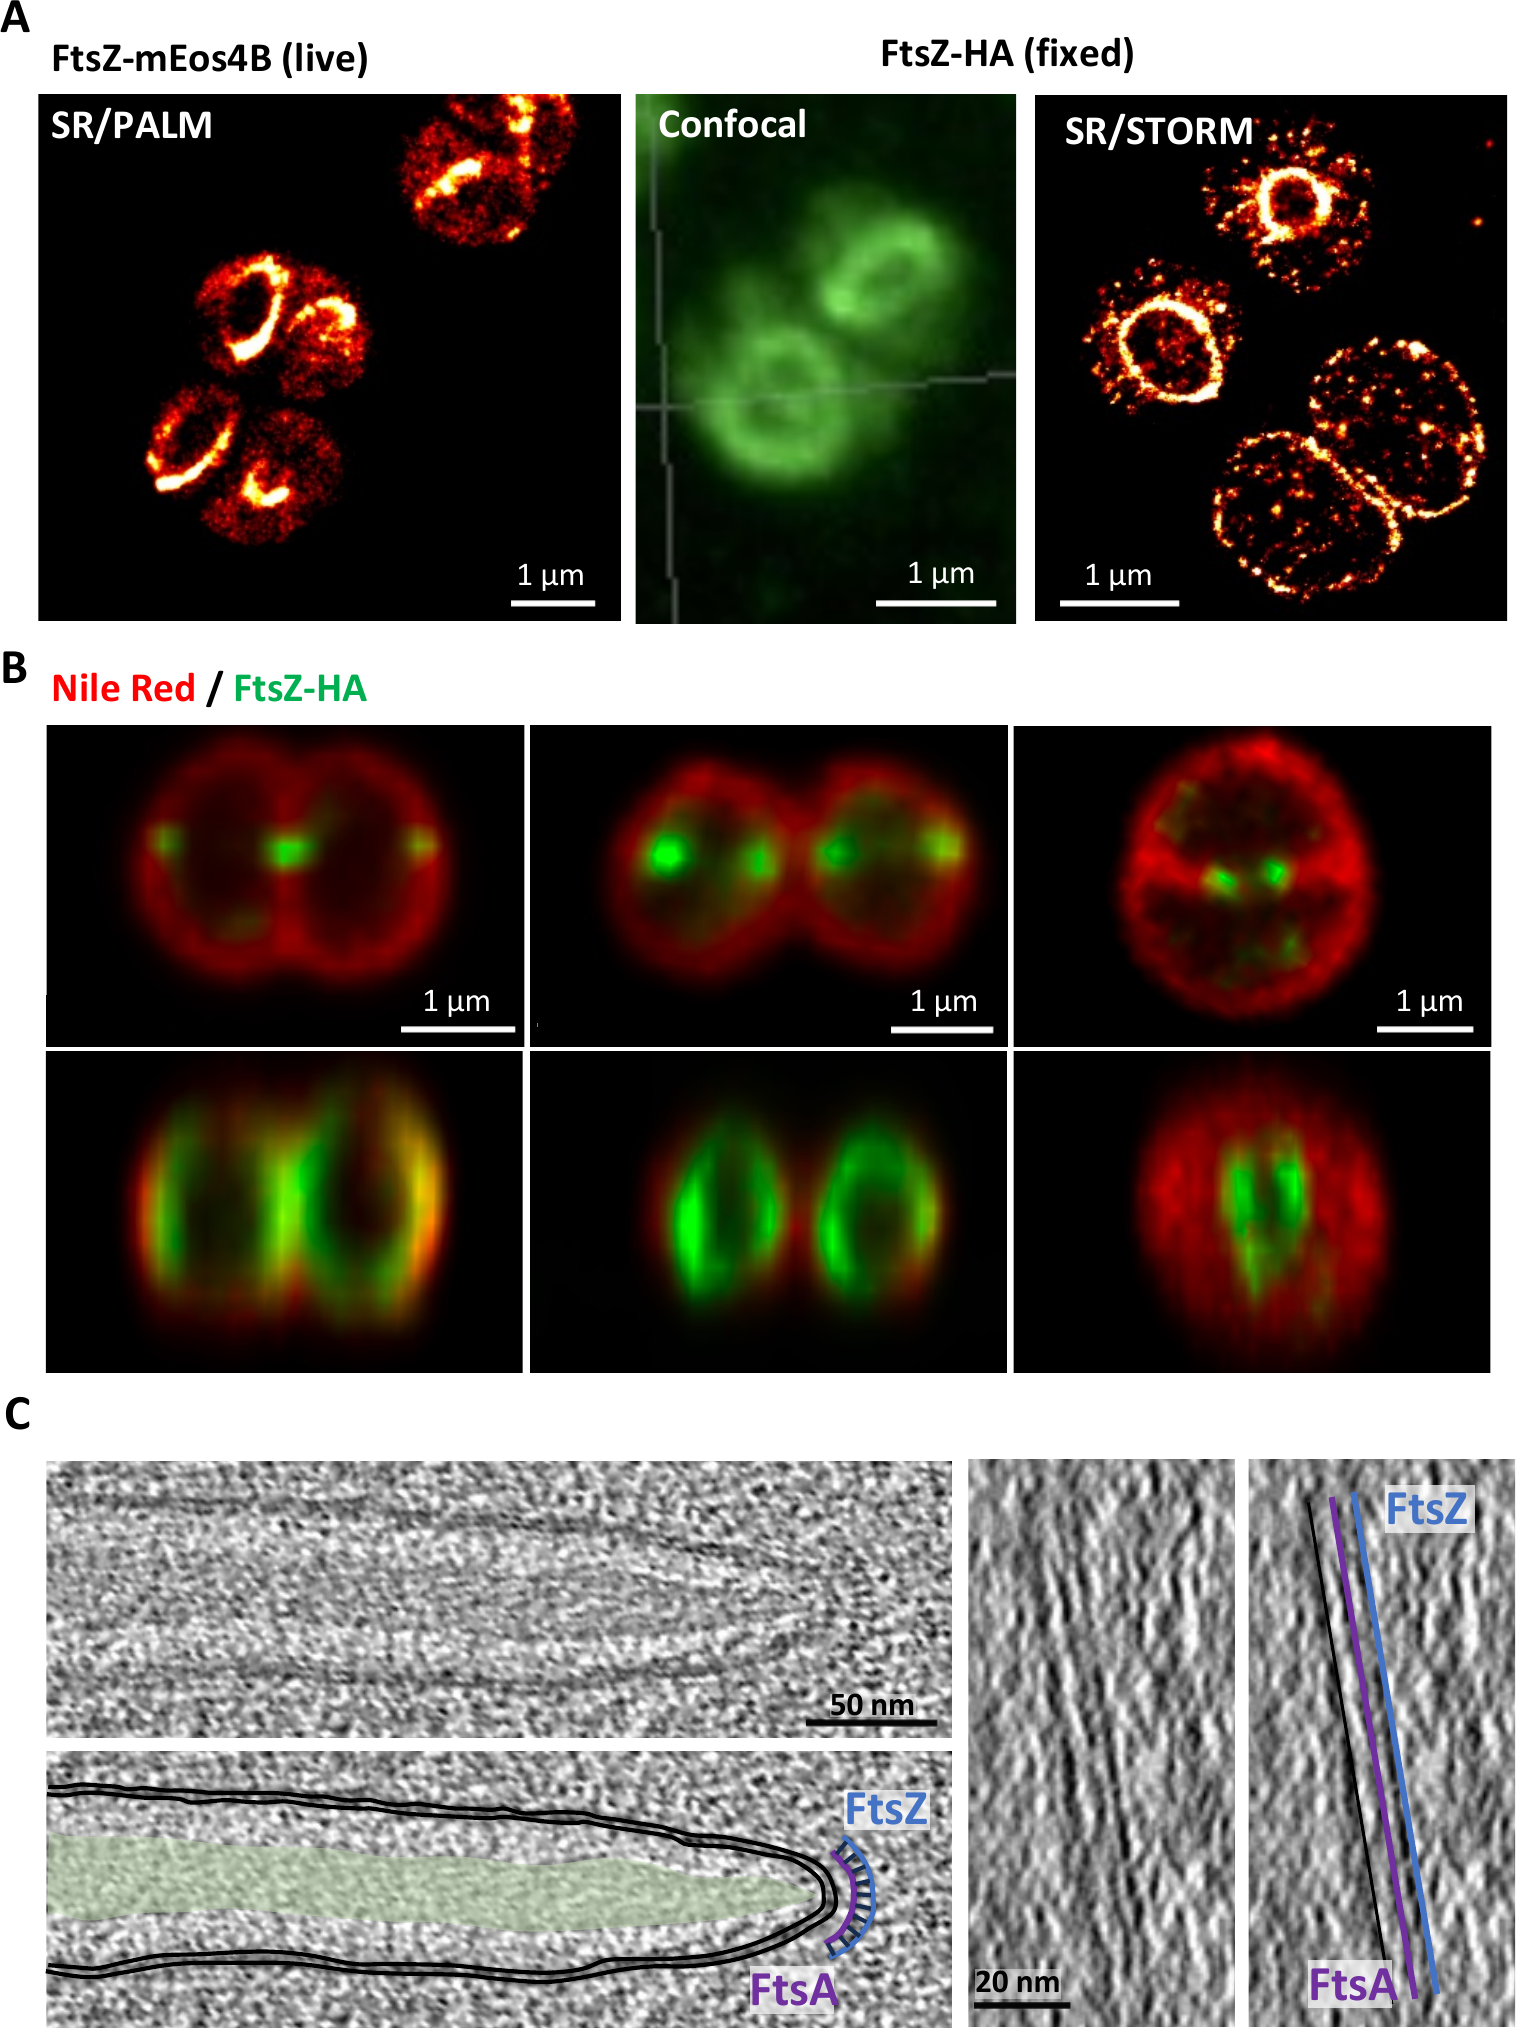
\includegraphics[width=.8\textwidth]{drad_paper/fig6.png}
    \titledcaption[Localisation of the key cell division factor, FtsZ, in D. radiodurans]{(caption on the next page)}
    \label{drad_fig6}
\end{figure}
\begin{figure}[ht]
    \ContinuedFloat
    \caption[]{(A) 3D fluorescence imaging of FtsZ in D. radiodurans. Left: 3D PALM imaging of D. radiodurans bacteria expressing FtsZ-mEos4B forming well-defined ring-like structures. Middle and right: 3D confocal images (middle) and super-resolved dSTORM images (right) of immunolabelled D. radiodurans bacteria expressing FtsZ-HA. Z-rings of various sizes and shapes were observed. Scale bar: 1 \mu{}m. (B) Two-colour labelling of D. radiodurans bacteria expressing FtsZ-HA. FtsZ (green) was immunolabelled while the membrane was stained with Nile Red (red). From left to right: illustrations of different stages of the division process. At all stages, FtsZ localizes to the leading edge of the septa. Top panels: top views, lower panels: side views. Scale bar: 1 \mu{}m. (C) Left: Averaged 2D slice from a typical tomogram of D. radiodurans illustrating the double-arched structure of FtsA (purple) and FtsZ (blue) located ~15 nm away from the IM bilayer (black) on the cytoplasmic side of the growing septum. The top panel shows an averaged 2D slice through of a tomogram and the lower panel the same region with segmentations of the various cell wall layers (colors as in Fig. 2A) and the double-arched structure. Scale bar: 50 nm. Right: Side-view of the FtsZ filaments highlighted in the right panel in blue. Inter-filament distance was estimated to be approximately 5 nm. Scale bar: 20 nm.}
\end{figure}

Examination of the tomograms revealed the presence in several of the tomograms (12 of the 45 tomograms) of a double-arched structure situated in the cytoplasm at \sim\qty{15}{nm} from the IM border of the leading edge of the septum, which likely corresponds to FtsZ (outer arch) and its cellular partner, the membrane-bound FtsA~\cite{sextonSuperresolutionConfocalCryoCLEM2022} (inner arch; \autoref{drad_fig6}C).
These two arches follow the curvature of the septal tip with the outer FtsZ arch typically between \qty{20}{nm} and \qty{50}{nm} in length.
As in our fluorescence microscopy data, these structures were observed at all stages of the septation process from budding septa all the way to almost fusing septa.
When looking at side-projections, FtsZ was found to form long straight parallel filaments along the flat leading edge of the closing septa with an inter-filament distance of approximately \qty{5}{nm} in good agreement with previous reports of \textit{in situ} FtsZ filaments~\cite{liStructureFtsZFilaments2007,szwedziakArchitectureRingFormed2014} (\autoref{drad_fig6}C).
Interestingly, FtsZ was not detected when membrane protrusions were present at septal tips, but was sometimes seen either above or below these structures, forming a discontinuous filament, which may explain the incomplete ring structures observed by fluorescence microscopy (\autoref{drad_fig6}A-B).

\FloatBarrier

\section{Discussion}

In this study, we have combined live conventional and super-resolution fluorescence microscopy with \textit{in situ} cryo-ET imaging of \textit{D. radiodurans} to follow the process of septation in this relatively large, spherical bacterium at the highest possible spatial and temporal resolutions.
This work provides important insight into (i) the complex cell wall composition of this unusual Gram-positive bacterium and the various stages of its maturation, (ii) its distinct mode of septation involving a "sliding door" mechanism, and (iii) the molecular mechanisms underlying PG synthesis and the coordinated septal growth that ensures successful fusion of the septa originating from opposite sides of the cell.

\textit{D. radiodurans} is a spherical bacterium that is known to possess a unique cell envelope including an outer S-layer, which has been the object of numerous studies over the past decades~\cite{vonkugelgenMultidomainConnectorLinks2022,workMorphologyChemistryCell1968,rothfussInvolvementSlayerProteins2006,vonkugelgenInterdigitatedImmunoglobulinArrays2023,farciSDBCActiveQuenching2023,farciStructuredOrganizationDeinococcus2022,farciCryoEMStructureSlayer2022,farciStructuralAnalysisArchitecture2021,baumeisterThreedimensionalStructureRegular1986,baumeisterStructureCellEnvelope1981}.
Like other members of the \textit{Deinococcus-Thermus} phylum, \textit{D. radiodurans} exhibits features of both Gram-positive and Gram-negative bacteria, and may be considered as a primitive form of Gram-negative bacteria~\cite{ericksonHowBacterialCell2017}.
\textit{D. radiodurans} is indeed lacking lipopolysaccharides typically found in Gram-negative bacteria, possesses a thick PG layer (35-55 nm) characteristic of Gram-positive bacteria and yet its cell envelope is composed of two membrane bilayers characteristic of Gram-negative bacteria~\cite{guptaOriginDidermGramnegative2011}.
The exact composition and structure of this unusual cell wall has been the object of much controversy in the recent years, notably regarding the outer layers linking the PG to the outermost S-layer hexagonal lattice structure.
Our cryo-ET analysis of the outer cell wall composition fully supports the model recently proposed by Bharat and colleagues, in which the whole outer cell envelope is \sim\qty{100}{nm} in thickness and composed of two membranes in between which can be found a thin periplasmic space and two thicker layers, the PG and SlpA layers~\cite{vonkugelgenMultidomainConnectorLinks2022}.
The S-layer forms an additional coat located \sim\qty{18}{nm} above the outer membrane~\cite{vonkugelgenInterdigitatedImmunoglobulinArrays2023}.
The SlpA layer takes its name from the major protein constituent of this layer, the SlpA protein, a trimeric porin-like protein that is embedded in the outer membrane and stretches across the SlpA layer via a long coiled-coil region to connect to the PG layer~\cite{vonkugelgenMultidomainConnectorLinks2022}.
The predicted length of this assembly (\sim\qty{28}{nm}-\qty{29}{nm}) is in good agreement with our estimated thickness of the SlpA layer (\qty{35}{nm}).
Interestingly, in our tomograms, we observe a distinctive white line between the PG and SlpA layers that may correspond to the sites at which the flexible N-terminal SLH domain of SlpA attaches to the PG layer.

In \textit{D. radiodurans}, daughter cell separation driven by the activity of autolysins~\cite{vermassenCellWallHydrolases2019} (four of which have been identified in \textit{D. radiodurans}~\cite{santosInterplayMnFe2019}) is uncoupled from septation, with these two phenomena occurring in successive cell cycles.
This is different from previously studied models of bacterial cell division in which both processes occur at the same time to produce two daughter cells.
Moreover, dividing \textit{D. radiodurans} cells exhibit three types of cell wall displaying distinct layer compositions and characteristics that reflect different stages of cell wall maturation.
The cell wall in the growing septa is initially composed of a central PG layer surrounded by a lipid bilayer, with a low-density periplasmic space in between these two layers.
The PG layer thickens progressively as the septa grow and this thickening continues after completion of the septation within the central septum.
The additional layers found exclusively in the outer envelope (SlpA layer and OM bilayer) are only added at a late stage of maturation when the splitting of the cells is initiated.
This differs from other bacteria and notably \textit{S. aureus} and \textit{E. coli} in which growing septa already exhibit two distinct PG layers (one for each daughter cell) separated by a low-density region~\cite{navarroCellWallSynthesis2022,matiasCryoelectronMicroscopyCell2007}.
This difference may be explained by the temporal separation between septation and cell splitting in \textit{D. radiodurans}, allowing PG hydrolysis and the synthesis of the two additional cell wall layers (and eventually the outer S-layer) to occur in the subsequent cell cycle within the central septum in a tightly coordinated manner.
First, the single thick PG layer found in this central septum region is separated through the action of hydrolases into two equal PG layers and the SlpA layer is synthesized in between these two PG layers before rapid synthesis of the OM bilayer to allow the incorporation of the abundant SlpA protein into both the OM and the SlpA layer.
These two additional layers efficiently protect \textit{D. radiodurans} from its external environment and must therefore be completed before the splitting of the daughter cells can take place.
The splitting process appears to be initiated from the outer boundaries of the cell at sites of outer membrane invagination and then moves inwards towards the center of the diad until full separation of the two daughter cells.

PG synthesis and its subsequent remodelling are key processes in bacterial septation.
In \textit{D. radiodurans}, PG synthesis has been shown to occur in both the septal regions and within the outer cell wall~\cite{flochCellMorphologyNucleoid2019}.
Here, by transiently incorporating aDA into the cell wall to label sites of active PG synthesis and remodelling~\cite{trouveNanoscaleDynamicsPeptidoglycan2021,lundMolecularCoordinationStaphylococcus2018}, we show that the leading edge of the septa constitutes the main site of PG synthesis in dividing \textit{D. radiodurans} and that subsequent rounds of synthesis build on the existing PG in an inwards direction until the opposing septa meet and fuse.
However, we also observed that the growing septa were very often tapered with a thinner PG layer at the leading edge than at the lagging edge.
This has previously been reported also in \textit{S. aureus}~\cite{giesbrechtStaphylococcalCellWall1998,matiasCryoelectronMicroscopyCell2007,lundMolecularCoordinationStaphylococcus2018} and suggests that PG synthesis may not be restricted to the leading edge of the septa.
In fact, the rapid loss of PG labelling within the growing septa during the chase phase of our aDA pulse-chase experiments suggests that septal PG is rapidly being remodelled and modified in this region.
In contrast, aDA incorporation within the outer cell wall was more stable, suggesting also that different machineries may be at a play in these two regions of cell wall.
This was further confirmed by our timelapse experiments performed in the presence of ampicillin, a \beta-lactam antibiotic that is known to specifically inhibit certain classes of PBPs.
As has been reported for the ovococci, \textit{Lactococcus lactis}~\cite{perez-nunezNewMorphogenesisPathway2011} and \textit{Streptococcus pneumoniae}~\cite{landRequirementEssentialPbp2x2013,kocaogluProfilingVlactamSelectivity2015}, we found that ampicillin treatment specifically impedes septation and not outer cell wall expansion needed for cell growth.
In ovococci, this effect has been attributed to the specific inhibition of the class B PBP, PBP2x, that is involved in septation~\cite{perez-nunezNewMorphogenesisPathway2011,landRequirementEssentialPbp2x2013,zapunPenicillinbindingProteinsBetalactam2008}.
The genome of \textit{D. radiodurans} encodes for two class A PBPs and one class B PBP, that is annotated as PBP2 (DR1868).
Although little is known so far about the respective roles of these PBPs in \textit{D. radiodurans}, our observations suggest that \textit{D. radiodurans} PBP2 may be the target of ampicillin and thus largely responsible for PG synthesis at the leading edge of the growing septa.

Whereas in most cocci and ovococci studied so far, septation advances centripetally from the outer cell wall like a closing diaphragm, with this study, we provide further evidence that septation in \textit{D. radiodurans} is quite distinct.
It proceeds via a "sliding door" mechanism, also described in an earlier study as a "septal curtain"~\cite{murrayCellDivisionDeinococcus1983}, in which the two septa originating from opposite sides of the cell grow inwards with a flat leading edge creating a central gap stretching from the top to the bottom of the cell.
As septation progresses, the leading edge becomes more curved and eventually when the two septa come close to each other, fusion occurs and the septal disk is filled.
Why \textit{D. radiodurans} uses such a remarkable mode of septation remains to date a mystery.
Physical constraints associated with the relatively large size (2-3 \mu{}m in diameter) of \textit{D. radiodurans}, its cell morphology (diads and tetrads) or its mode of division in two alternating perpendicular planes may have contributed to the development of this unusual mode of division.

With such a septation process, ensuring the opposing septa are correctly aligned and meet at mid-cell for septal fusion constitute major challenges for the bacteria.
The latter is, in part at least, achieved by differential growth rates of the external and internal septa.
Indeed, we observed that the septum originating from the external side of the diad grows at a faster rate and initiates its growth shortly before the septum originating from the central septum to compensate for the longer distance needed for it to reach mid-cell.
This study also identifies two other important factors that may facilitate this process: (i) the flexible membrane protrusions observed at the leading edge of septa, and (ii) the presence of FtsZ at septal tips and the formation of Z-rings that may constitute a physical link between the opposing septa.

These two mutually exclusive features were indeed observed at the leading edge of \textit{D. radiodurans} septa.
In many instances, particularly at early stages of the septation process, membrane protrusions, adopting a variety of conformations, were observed at the tips of the growing septa.
Similar structures were reported in early studies of \textit{D. radiodurans}~\cite{thornleyFineStructureMicrococcus1965,sleytrStudyFreezeetchingFine1973} and other bacteria~\cite{suganumaStudiesFineStructure1966,pontefractMesosomesEscherichiaColi1969}, but were later considered as artefacts of chemical fixation procedures used for electron microscopy sample preparation~\cite{ryterContributionNewCryomethods1988,dubochetElectronMicroscopyFrozenhydrated1983,liedtkeHowAdvancesCryoelectron2022}.
In our case, these structures were observed \textit{in situ} in near native conditions (vitrified lamellae) strongly suggesting that they are not artefacts.
Instead, we propose that these thin mobile membrane extensions, missing a PG layer, may provide the necessary flexibility to allow septa to align with their opposing septa during the initial steps of septation.
In contrast, the presence of FtsZ at the septal tips was associated with more rigid and well aligned septa, suggesting that the assembly of the FtsZ ring may constitute a critical step in the proper alignment of opposing septa, possibly through a direct bridging of the two "sliding doors".
Importantly, FtsZ was only observed at the leading edge of septa containing a well-defined central PG layer that extended almost to the lipid bilayer significantly reducing the low-density periplasmic space in these tips.
In addition to possibly bridging the opposing septa via its ring formation, FtsZ is likely also acting as an anchor for the recruitment of the PG synthesis machinery needed for septation, as has been reported for many other bacteria (recently reviewed in~\citet{barrowsFtsZDynamicsBacterial2021,mcquillenInsightsStructureFunction2020,cameronInsightsAssemblyRegulation2024}).

Although FtsZ was never seen on the membrane protrusions themselves, in several tomograms FtsZ was observed either above or below the protrusions.
The leading edge of a given "sliding door" may thus be heterogeneous composed of both flexible regions bearing membrane protrusions and more rigid areas in which FtsZ can assemble to drive PG synthesis.
We thus propose a model for \textit{D. radiodurans} septation (\autoref{drad_fig7}) in which membrane synthesis may precede PG synthesis during the early stages of septation, leading to the formation of membrane protrusions.
The subsequent assembly of FtsZ filaments at the leading edge of the septa followed by the formation of the Z-ring would then act as a cue for the recruitment and activation of PG synthesis in order to progressively fill and rigidify the growing septa.
Further studies will certainly be needed to decipher the precise roles of FtsZ and to identify the other key players in this complex and intriguing septation process.

\begin{figure}[ht]
    \centering
    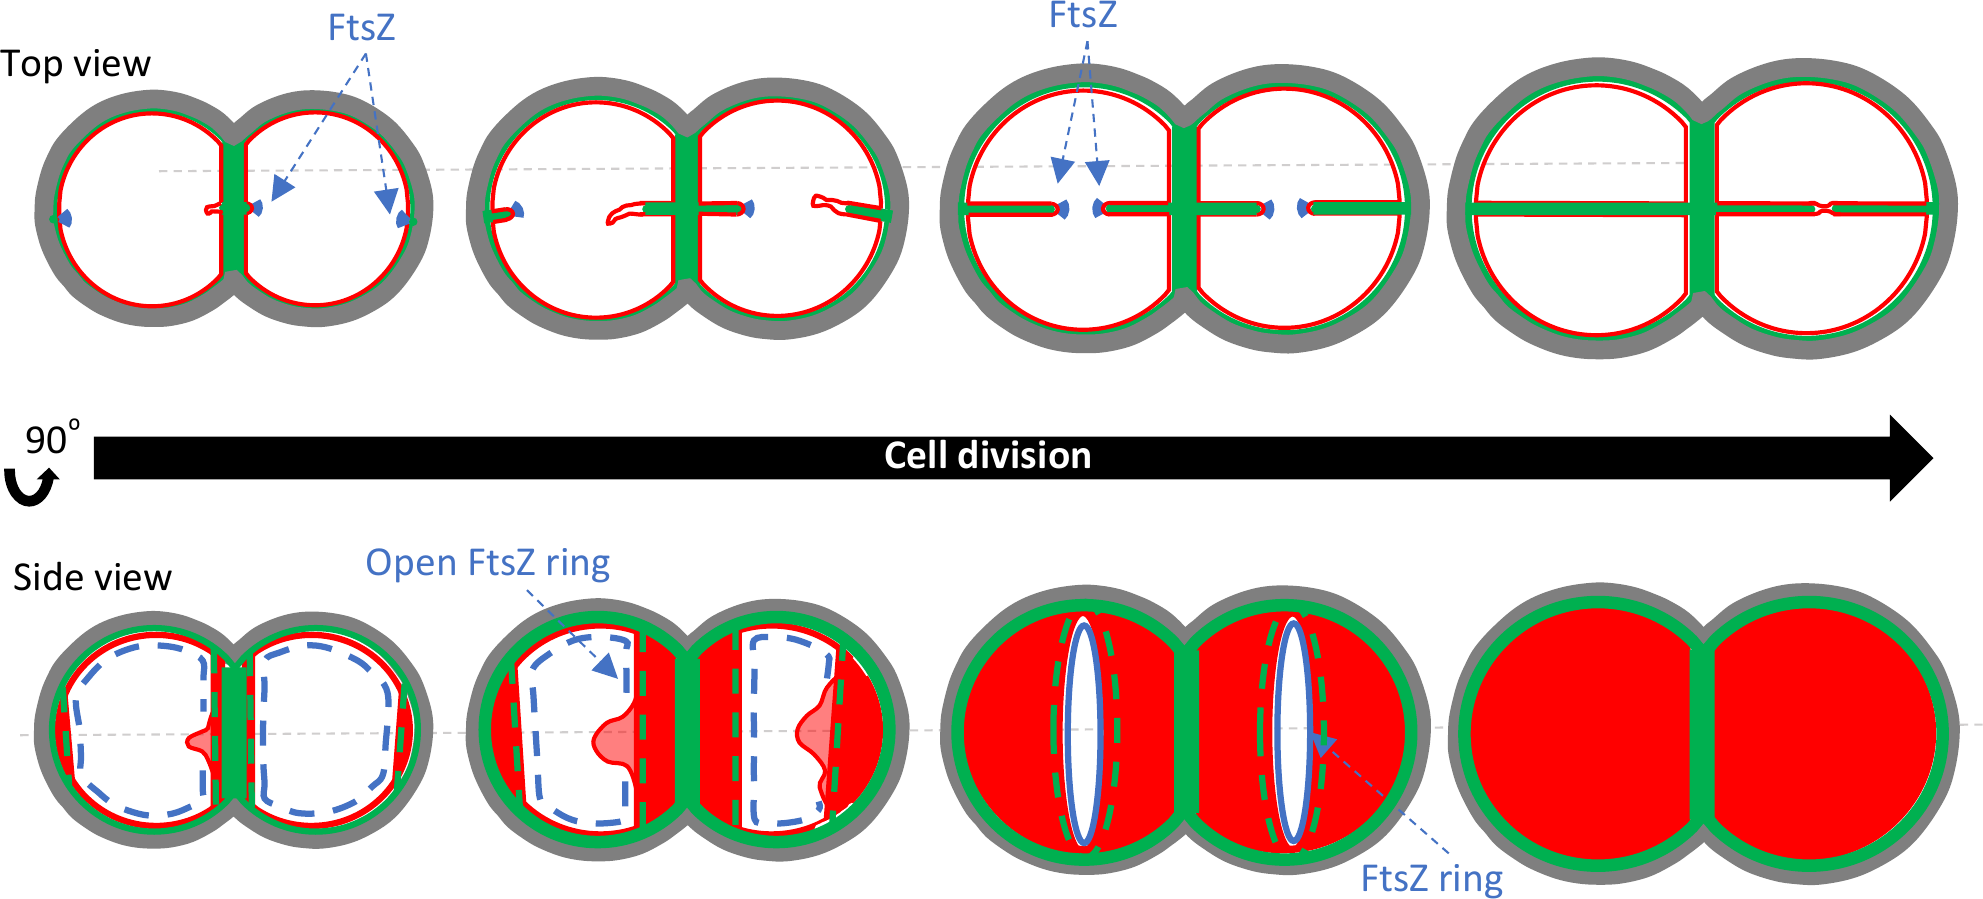
\includegraphics[width=\textwidth]{drad_paper/fig7.png}
    \titledcaption[Schematic model of the septation process in D. radiodurans]{Top and side views are illustrated at various stages of the division process. For simplicity, only the IM (red) and the PG layer (green) are highlighted. FtsZ is shown in blue with incomplete Z-rings as dashed lines and complete Z-rings as a full line. Flexible membrane protrusions are visible at early stages of the septation process, which progressively become filled with PG providing the necessary rigidity to achieve a solid and well-aligned cross-wall. FtsZ plays a key role in targeting the PG synthesis machinery to the leading edge of the growing septa and may also facilitate the proper alignment of opposing septa by bridging the two independent elements via Z-ring formation.}
    \label{drad_fig7}
\end{figure}

\section{Materials \& Methods}

\subsection{Bacterial cultures}

\textit{D. radiodurans} (DR) strains used in this study are listed in Table S1.
All strains were derivatives of the wild-type strain R1 ATCC 13939 (DR\textsuperscript{WT}).
The genetically engineered strain of \textit{D. radiodurans} expressing FtsZ fused to mEos4B (DR-\textit{FtsZ-mEos4B}) was obtained by the tripartite ligation method as described recently~\cite{vauclareStressinducedNucleoidRemodeling2024}.
A synthetic gene encoding mEos4B was amplified together with the kanamycin resistance cassette by PCR as were the regions (\sim500bp) flanking the insertion site (3' end of \textit{ftsZ} gene and region immediately downstream of the \textit{ftsZ} gene) using oligonucleotides listed in Table S2.
After restriction digestion the three fragments were ligated together and transformed into \textit{D. radiodurans}.
Transformants were selected on TGY agar plates containing \qty{6}{\mu{}g/ml} kanamycin, leading to allelic replacement on one genome copy.
Because \textit{D. radiodurans} is multigenomic, the transformant colonies were streaked three times successively on selective medium to ensure that all copies of the genome had incorporated the foreign DNA.
This was then confirmed by PCR analysis and DNA sequencing.
\textit{D. radiodurans} cells were grown aerobically at \ang{30}C in a shaking incubator (160 rpm) in Tryptone-Glucose-Yeast extract 2x (TGY2X) medium supplemented with the appropriate antibiotics.
Typically for microscopy experiments, \textit{D. radiodurans} cells were pre-grown the day before and then diluted for an overnight growth until reaching exponential (OD\textsubscript{650} \sim0.3-0.5) the next morning.
Optical density measurements were made on a Clariostar (BMG Labtech) plate reader.

\subsection{Cell labelling for confocal and single-molecule localization (SMLM) microscopy}

Membranes of exponential phase DR bacteria were stained by addition of Nile Red (30 \mu{}M for confocal microscopy and 30-100 nM for SMLM) to the growth medium of cells (1 ml) for 10 min at room temperature.
The cells were then harvested by centrifugation and resuspended in 200 \mu{}l TGY2X for confocal microscopy or instead washed 3 times in DPBS (3x 1 ml) and resuspended in 200 \mu{}l DPBS for SMLM.
3-5 \nu{}l of cell suspension was then deposited on a 1.5\% (w/v) low melting agarose (LMA; Bio-Rad) pad prepared using a gene frame positioned on a glass slide.
Two stripes of LMA were cut out on either side of the deposited sample for good aeration of the bacteria before a 1.5H coverslip was added to cover the frame.
For PALM imaging of FtsZ-mEos4B, DR-\textit{FtsZ-mEos4B} cells were grown to exponential phase, washed twice with DPBS and deposited directly on a 1.5\% LMA pad prepared in DPBS using a gene frame positioned on a glass slide.
To visualize dividing bacteria in different orientations, an alternative set-up was also used (\autoref{drad_sfig1}B) in which 10 \mu{}l of the cell suspension was placed on the bottom of a glass dish and cells were allowed to sediment for 2 min.
Excess liquid was then gently removed using a pipette and after 2 minutes of air-drying, 10 \mu{}l 1.5\% LMA equilibrated at \ang{37}C was poured over the cells.
The LMA was prepared in TGY2X medium for timelapse confocal imaging and in DPBS for PAINT imaging of Nile Red labelled bacteria.
For PG labelling, 1.5 ml of exponential phase DR cultures were centrifuged at 3000xg and resuspended in 200 \mu{}l TGY2X medium to which 50 \mu{}l 10 mM azido-D-Alanine (aDA) was added~\cite{trouveNanoscaleDynamicsPeptidoglycan2021,trouveMetabolicBiorthogonalLabeling2021}.
Pulse labelling was typically performed for 10 min at \ang{30}C, before washing the cells two times with cold DPBS to stop cell growth.
Cells were then resuspended in 48 \mu{}l 30 \mu{}M DBCO-AF488 or DBCO-AF647 (dSTORM) diluted in DPBS and incubated on ice for 45 min to allow the DBCO-AF488/AF647 to enter the bacteria and react by click chemistry with the incorporated aDA.
When ready to be imaged, labelled cells were washed two times with DPBS and resuspended in 100 \mu{}l DPBS.
For immunolabelling of HA-tagged FtsZ, DR-\textit{FtsZ-HA} (strain GY15705) bacteria were grown to exponential phase.
0.5 ml culture was flash-frozen using liquid nitrogen in DPBS-glycerol buffer (19\% glycerol) supplemented with 2.58\% formaldehyde.
Cells were then fixed through slow thawing of these samples on ice overnight, washed twice in DPBS and resuspended in 100 \mu{}l DPBS.
Cells were permeabilized by treatment with 4 mg/ml lysozyme at \ang{37}C for 30 min followed by the addition of 0.1\% Triton X-100 for 5 min at \ang{25}C.
Cells were then washed twice with DPBS and incubated with a mouse anti-HA antibody (1:400 dilution in PBS-Tween0.05\% supplemented with 2\% BSA) for 1h at \ang{37}C.
After several washes with PBS-Tween0.05\%, cells were incubated with anti-mouse secondary antibody coupled to either Alexa fluor 488 (for confocal) or Alexa Fluor 647 (for dSTORM) for 1h at \ang{37}C.
After a final washing step, the bacteria were deposited on a 1.5\% LMA pad prepared in DPBS as described above.
For dSTORM experiments, the LMA was prepared in glucose buffer (62.5 mM Tris-HCl pH 8.0, 12.5\% glucose, 12.5 mM NaCl) and contained 0.1M MEA and 1x GLOX (prepared from the 10x GLOX solution composed of 10 mM Tris-HCl pH 8.0, 50 mM NaCl, 56 mg/ml Glucose oxidase and 13.6 mg/ml Catalase).
For confocal microscopy, the LMA was prepared as above in TGY2X.

\subsection{Confocal data acquisition and processing}

Spinning-disk confocal microscopy was performed using an Olympus IX81 inverted microscope equipped with a Yokogawa CSU-X1 confocal head.
The excitation laser beam (Ilas2 laser bench, GATACA systems) was focused to the back focal plane of a 100X 1.49-numerical-aperture (NA) oil immersion apochromatic objective.
Series of Z-planes were acquired every \qty{132}{nm} using a PRIOR N400 piezo stage to achieve cubic voxels.
Fluorescence excitation was performed at \qty{488}{nm} for DBCO-AF488 and \qty{561}{nm} for Nile Red.
Fluorescence emission was collected with an Andor iXon Ultra EMCCD camera through a quad-band Semrock\texttrademark Di01-T405/488/568/647 dichroic mirror and single-band emission filters adapted to each fluorophore used: \qty{520}{nm} for DBCO-AF488 (FF02-520/28 Semrock\texttrademark), and \qty{600}{nm} for Nile Red (ET600/50m Chroma\texttrademark).
Data acquisition was performed using Metamorph 7.10 (Molecular devices).
Acquired images were processed using Imaris (Oxford Instrument\texttrademark) to correct for the possible translational (in x, y, and z directions) and rotational (z axis) drifts, followed by correction of the timepoints intensities using the embedded "Normalized timepoint" routine (Imaris XT package).
When needed, Kymograph builder plugin in Fiji was applied to datasets.
Coordinates of kymograph boundaries were then extracted in Fiji and used to calculate the septal closure rate in growing cells.

\subsection{SMLM (PAINT/dSTORM) data acquisition and processing}

PAINT and dSTORM data were acquired on an Olympus IX83 inverted motorized microscope equipped with a SAFE 360 (Abbelight) SMLM set up, and using a UPLXAPO 100x oil immersion objective (1,5NA, Olympus\texttrademark).
Data collection was performed using simultaneous dual camera acquisitions (50/50 splitter; Orca Fusion sCMOS -- Hamamatsu\texttrademark) with an astigmatism lens intercalated in the emission path of the direct camera to reconstruct 3D volumes in parallel with 2D single-molecule localization determination.
Data was acquired at \ang{27}C under continuous HiLo illumination with 400 W/cm² 561 nm light or 642 nm light and a typical frame time of 10 ms for PAINT and 50 ms for dSTORM.
Typically, 40,000 -- 60,000 frames were acquired per dataset under constant activation of the Zero Drift Control system (ZDC2 at 830 nm) to limit Z-drift during acquisitions, and at constant temperature (Digital Pixel\texttrademark blind cage incubator and water jacket around the objective set at \ang{27}C).
Typical 3D reconstructions are limited by the astigmatic point spread function to a few hundreds of nm.
When specified in the corresponding figure legends, we collected stacked localizations at 400 nm distance and reconstructed the cumulated localizations to obtain larger reconstructed volumes.
SMLM data was processed using NeoAnalysis software (Abbelight\texttrademark) using default values for maximum likelihood estimations (MLE) of the gaussian localizations fittings.
Further filtering of the dataset was performed using Thunderstorm plugin~\cite{ovesnyThunderSTORMComprehensiveImageJ2014} in Fiji~\cite{schindelinFijiOpensourcePlatform2012} to correct for possible drift in x and y directions (using cross-correlation), and restrict the localizations to limit the spreading of values for sigma, intensity, and uncertainty values.

\subsection{Sample preparation, vitrification and cryo-FIB milling for cellular cryo-ET}
A 20 ml pre-culture of \textit{D. radiodurans} cells was grown overnight to stationary phase (OD\textsubscript{650} \sim1.8) in TGY2X medium in a shaking incubator at \ang{30}C and 170 rpm and then diluted to OD\textsubscript{650} \sim0.1 in XXX ml fresh medium the next day and grown further until reaching exponential phase (OD\textsubscript{650} \sim0.4).
The culture was then centrifuged for 5 min at 4000 rpm, the pellet collected in a 1 ml Eppendorf tube and washed three times in 1 ml PBS.
Shortly before plunge-freezing, the pellet was resuspended in PBS to reach a final volume of \sim60 \mu{}l.
Plunge-freezing was performed in liquid ethane/propane mixture using Vitrobot Mark IV (Thermo Fisher Scientific) at \ang{23}C, 90\% humidity, with blot force -5 to 10, blot time 8 to 10 sec and wait time 30 sec.
4 \mu{}l of cell suspension were deposited per Quantifoil Cu 1.2/1.3, 200 mesh grid (Micro Tools GmbH, Großlöbichau, Germany), glow-discharged immediately prior to use.
Frozen grids were clipped into standard AutoGrid specimen cartridges (Thermo Fisher Scientific) marked to keep track of the milling direction for the subsequent orientation in the Titan Krios (ThermoFisher Scientific) microscope, and stored in liquid nitrogen until usage.
For cryo-FIB milling, the clipped grids were mounted into a \ang{45} pre-tilt shuttle and transferred into a Scios cryo-FIB/scanning electron microscope dual-beam microscope (Thermo Fisher Scientific).
To reduce curtaining and enhance sample conductivity, the grids were sputter-coated with organometallic platinum using the gas injection system.
The Gallium milling was performed at a \ang{17} to \ang{23} stage tilt angle, dependent on the milling location on the grid.
Lamellae were prepared in a stepwise manner, progressively reducing the FIB current from 0.5 nA to remove the bulk material to 30 pA for the final polishing step, ending up with lamellae of 200-300 nm thickness.
Progress of the milling process was monitored using the SEM operated at 10 kV and 50 pA.
Grids were stored in liquid nitrogen until transfer into the Titan Krios microscope.

\subsection{Cryo-ET data acquisition}
Data was collected using a Titan Krios operated at 300 keV and equipped with a BioQuantum post-column energy filter (Gatan, Pleasanton, CA) and a K2 Summit direct detector (Gatan, Pleasanton, CA).
The energy filter was operated with a 20 eV slit width.
Image acquisition was performed using SerialEM software.
To identify regions of interest (ROI) and account for the lamella pre-tilt, lamella montages were acquired at an intermediate magnification of 8700x (corresponding to XXX nm/pixel), and at +\ang{13} tilt.
Tilt series were then recorded with the detector operated in super-resolution mode, at a nominal magnification of 33,000x corresponding to \qty{2.173}{\angstrom/pixel} at the specimen level.
Data were collected at defocus of -XXX to -YYY \mu{}m following a grouped dose-symmetric tilt scheme in 3° increments, with a tilt range depending on the ROI position and thickness, typically \pm\ang{50} to \pm\ang{60}.
The dose was kept constant for all tilts in each given tilt series and adjusted such as to reach the total per tilt series dose of \sim\qty{140}{e/\angstrom}~\cite{ericksonHowBacterialCell2017}.
In total, 45 tilt series were collected for the presented analysis.
% TODO: fill in the XXX and YY above!

\subsection{Cryo-ET image processing, visualization, segmentation and analysis}
Data preprocessing was carried out in Warp~\cite{tegunovRealtimeCryoelectronMicroscopy2019}: gain reference and motion correction, and CTF estimation were performed following the standard Warp~\cite{tegunovRealtimeCryoelectronMicroscopy2019} procedure for tomography data with the following non-default parameters: binning 1x, CTF grid dimensions 5x5x1, and motion grid dimensions 5x5x15.
The dataset was then manually curated to remove low quality tilt images and extracted into stacks for tilt series alignment.
Alignment was performed in batch with AreTomo~\cite{zhengAreTomoIntegratedSoftware2022}, using our in-house script Waretomo (\href{https://doi.org/10.5281/zenodo.13350542}{source code}) to integrate it seamlessly with Warp~\cite{tegunovRealtimeCryoelectronMicroscopy2019}.
Alignment parameters were reimported in Warp~\cite{tegunovRealtimeCryoelectronMicroscopy2019} and used to reconstruct full tomograms at a resolution of \qty{17.41}{\angstrom/pixel}.
Tomograms were denoised using Topaz~\cite{beplerTopazDenoiseGeneralDeep2020} to help with picking and inspection.
All images of tomogram slices presented in this manuscript come from non-denoised tomograms, averaging over 5 slices.
Cell walls were annotated using the surface annotation tool in blik~\cite{gaifasBlikExtensible3D2024} (\href{https://zenodo.org/records/10894490}{source code}).
These annotations were then used to generate the 3D surface visualizations of the septa and cell wall profiles using the surface tool in blik~\cite{gaifasBlikExtensible3D2024}, resampling the tomogram perpendicularly to the surfaces to obtain "straightened" wall volumes.
2D projections were obtained by averaging over the Z dimension of the resampled volumes.
1D density profiles were calculated in Fiji~\cite{schindelinFijiOpensourcePlatform2012} on 76-pixel sections of the 2D projections and used to measure cell wall dimensions using the point to point measuring tool in Fiji~\cite{schindelinFijiOpensourcePlatform2012} as detailed in \autoref{drad_sfig8}.

\section{Acknowledgements}
IBS acknowledges integration into the Interdisciplinary Research Institute of Grenoble (IRIG, CEA).
This work used the M4D imaging platform of the Grenoble Instruct-ERIC center (ISBG ; UAR 3518 CNRS-CEA-UGA-EMBL) within the Grenoble Partnership for Structural Biology (PSB), supported by FRISBI (ANR-10-INBS-0005-02) and GRAL, financed within the University Grenoble Alpes graduate school (Ecoles Universitaires de Recherche) CBH-EUR-GS (ANR-17-EURE-0003).
We thank staff on the M4D platform at IBS and from the Umeå Centre for Electron Microscopy for their help for data acquisition and processing.

\section{Funding}
This work benefitted from funding from the CEA Radiobiology program and the Agence Nationale de la Recherche (grant N~\textsuperscript{o} ANR-22-CE11-0029-01).
LG's PhD position was funded by GRAL, a project of the University Grenoble Alpes graduate school (Ecoles Universitaires de Recherche) CBH-EUR-GS (ANR-17-EURE-0003).
% TODO Funding for sabbatical in Sweden??

\newpage

\section{Supplemental Figures}

\begin{figure}[ht]
    \centering
    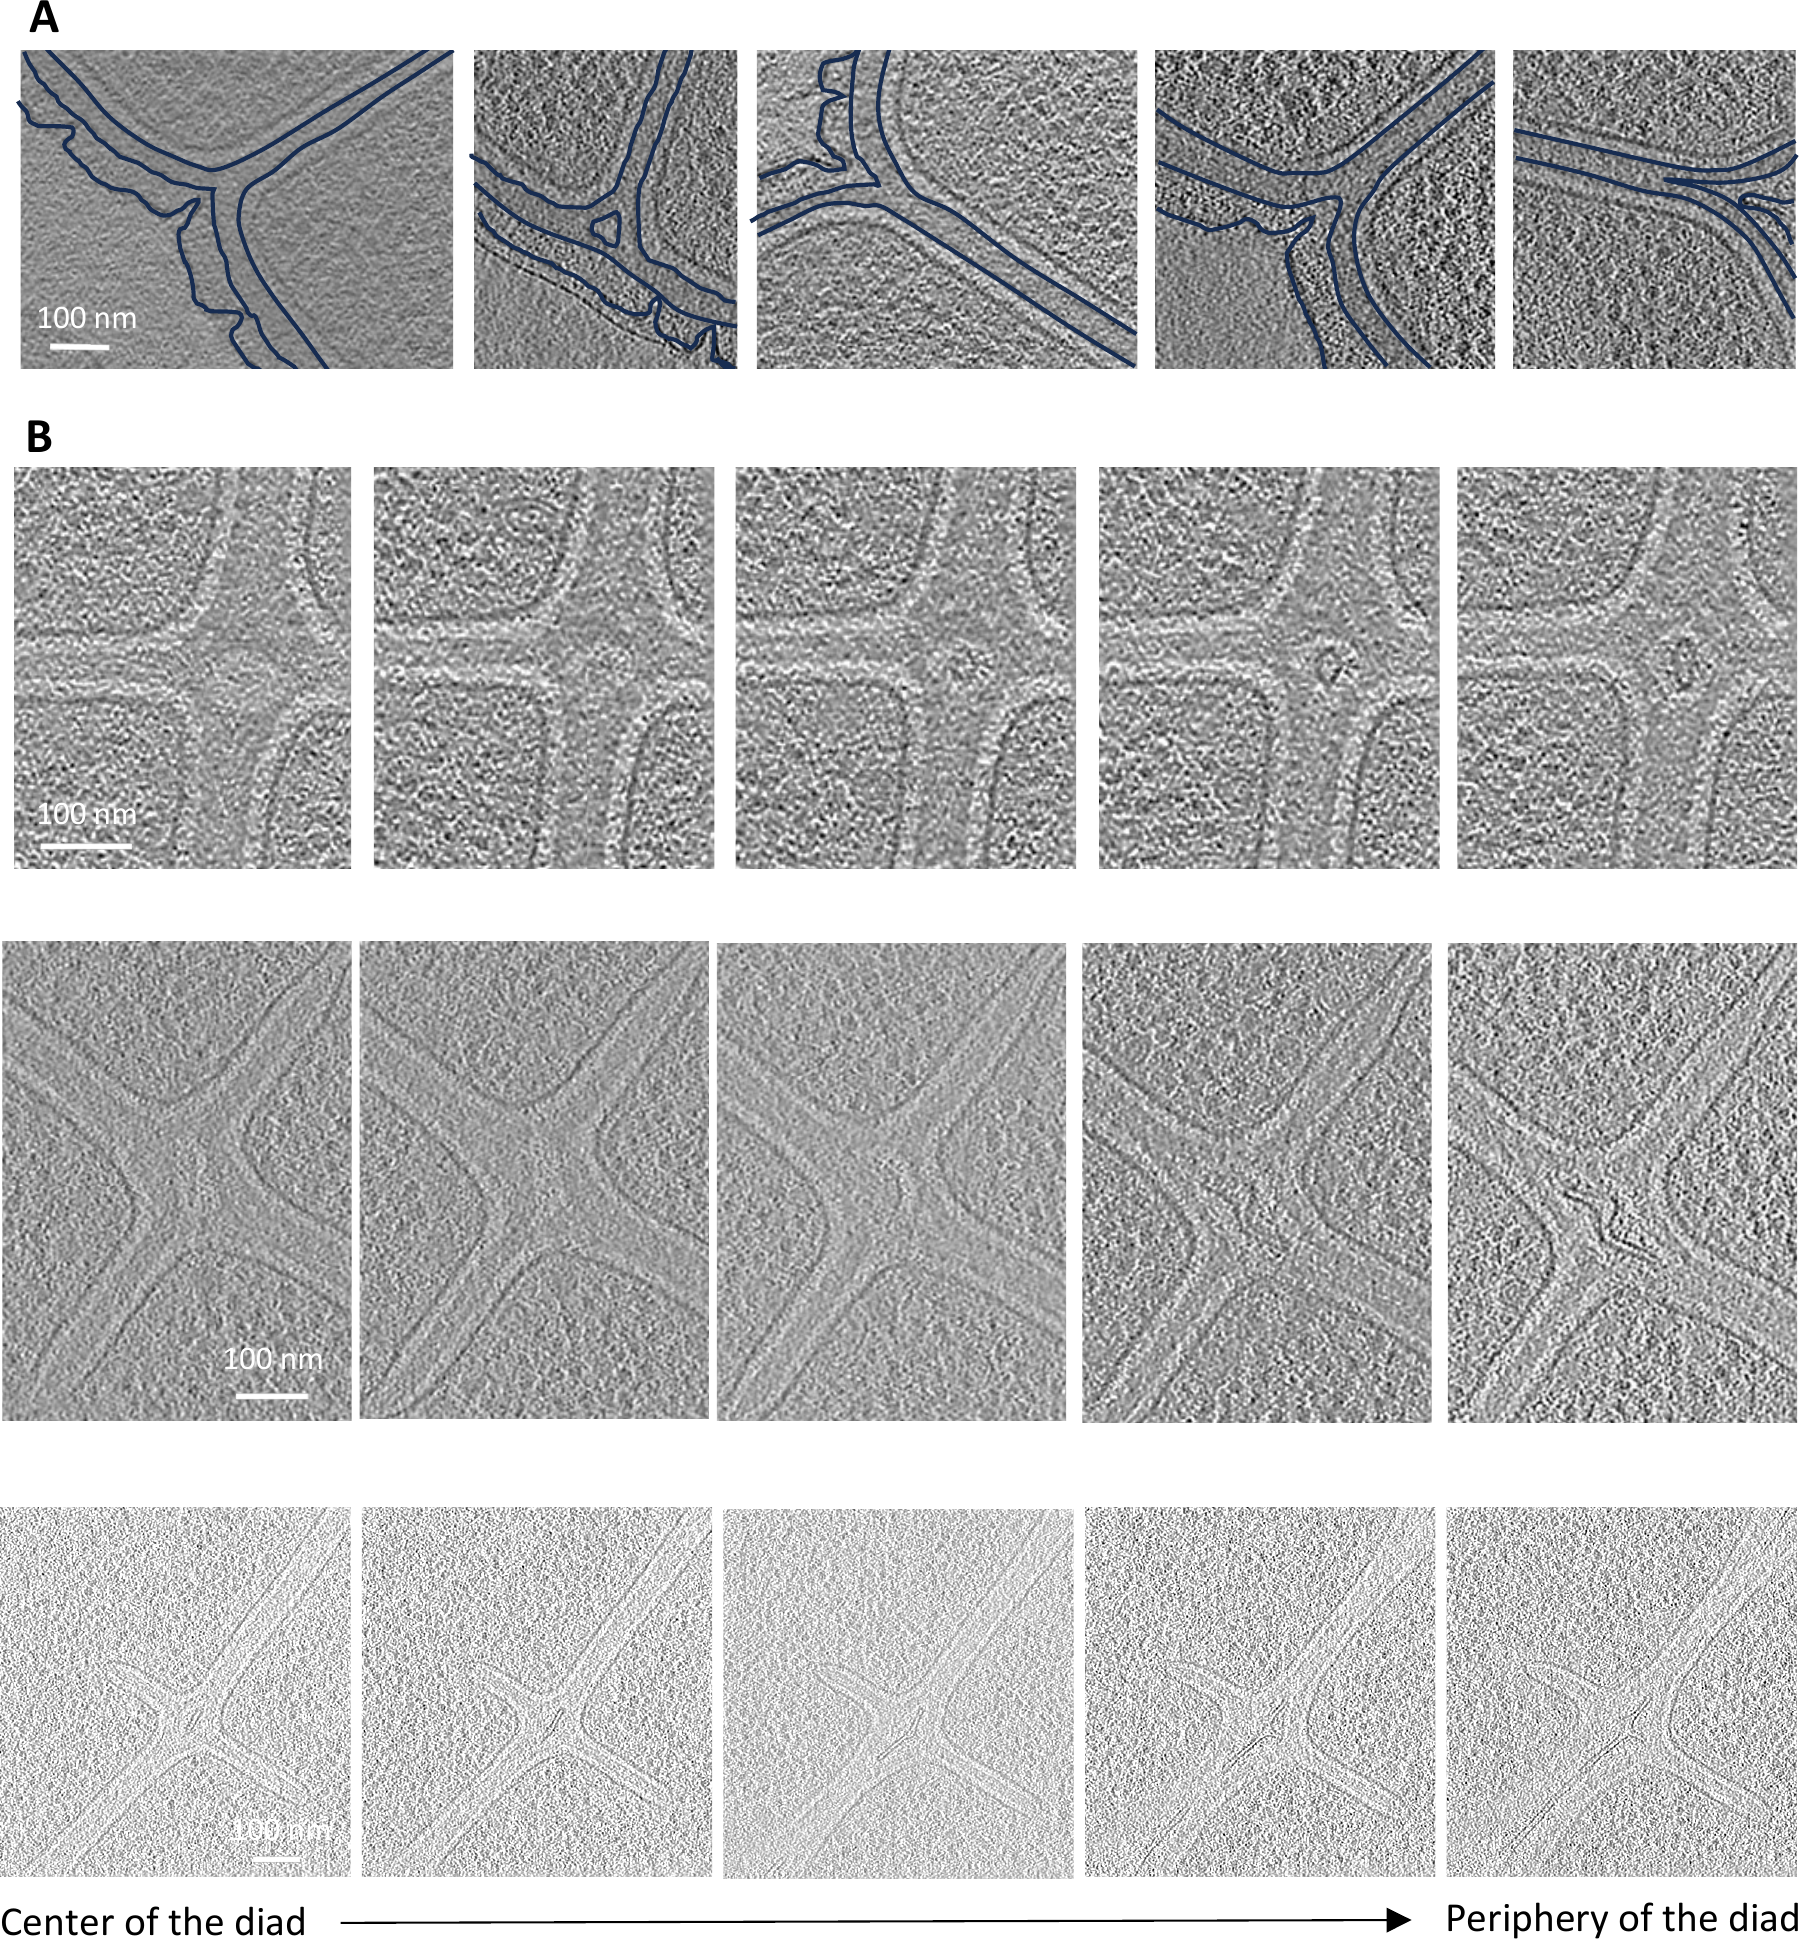
\includegraphics[width=\textwidth]{drad_paper/sfig1.png}
    \titledcaption[Cell wall junction examples]{(A) Examples of junctions between the outer cell wall and the growing septa observed in various tomograms of D. radiodurans. The borders of the different layers composing the cell wall are highlighted in dark blue. (B) Examples of regions in which splitting of the daughter cells were observed. From left to right: slices through the tomograms with the earlier stages of cell splitting illustrated on the left (located towards the center of the diads) and the later stages on the right (located closer to the outer periphery of the bacteria).}
    \label{drad_sfig1}
\end{figure}

\begin{figure}[ht]
    \centering
    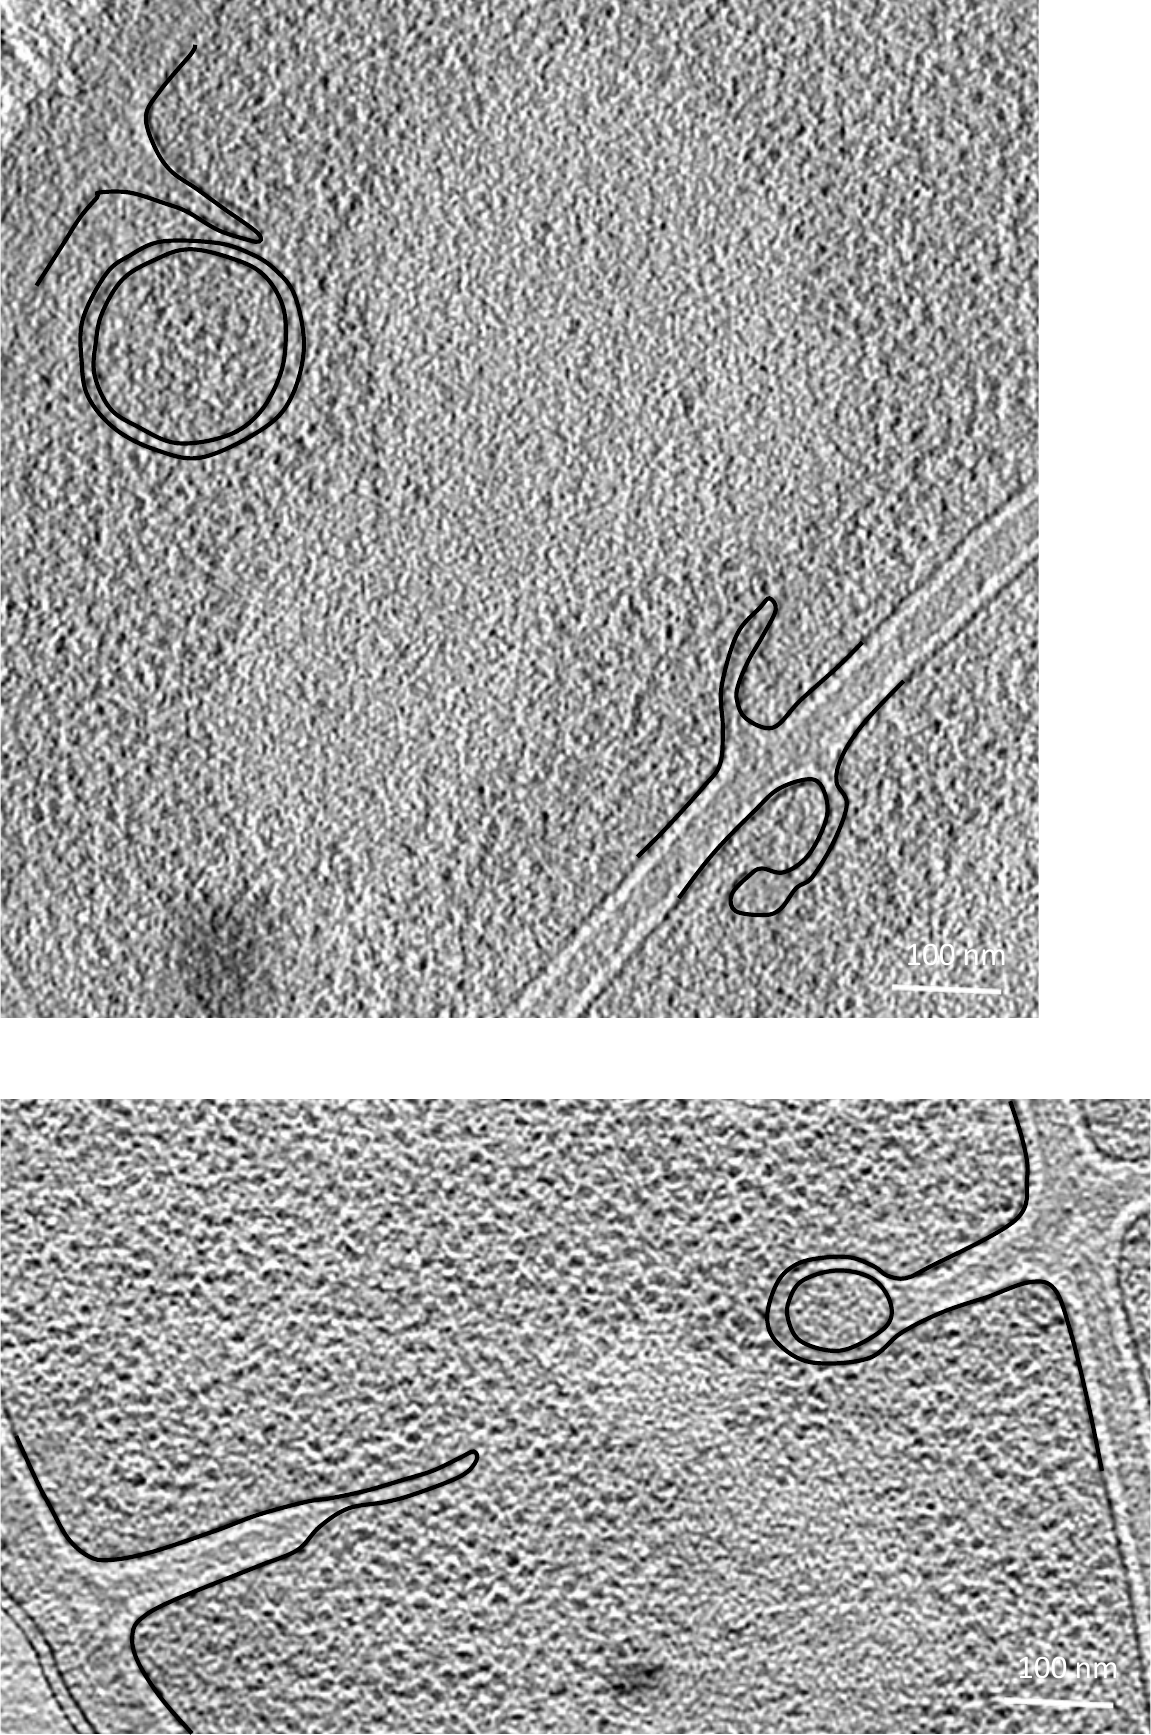
\includegraphics[width=.8\textwidth]{drad_paper/sfig2.png}
    \titledcaption[Membrane protrusion examples]{Examples of membrane protrusions observed in various tomograms of D. radiodurans at the leading edge of growing septa. The IM is highlighted in black.}
    \label{drad_sfig2}
\end{figure}

\begin{figure}[ht]
    \centering
    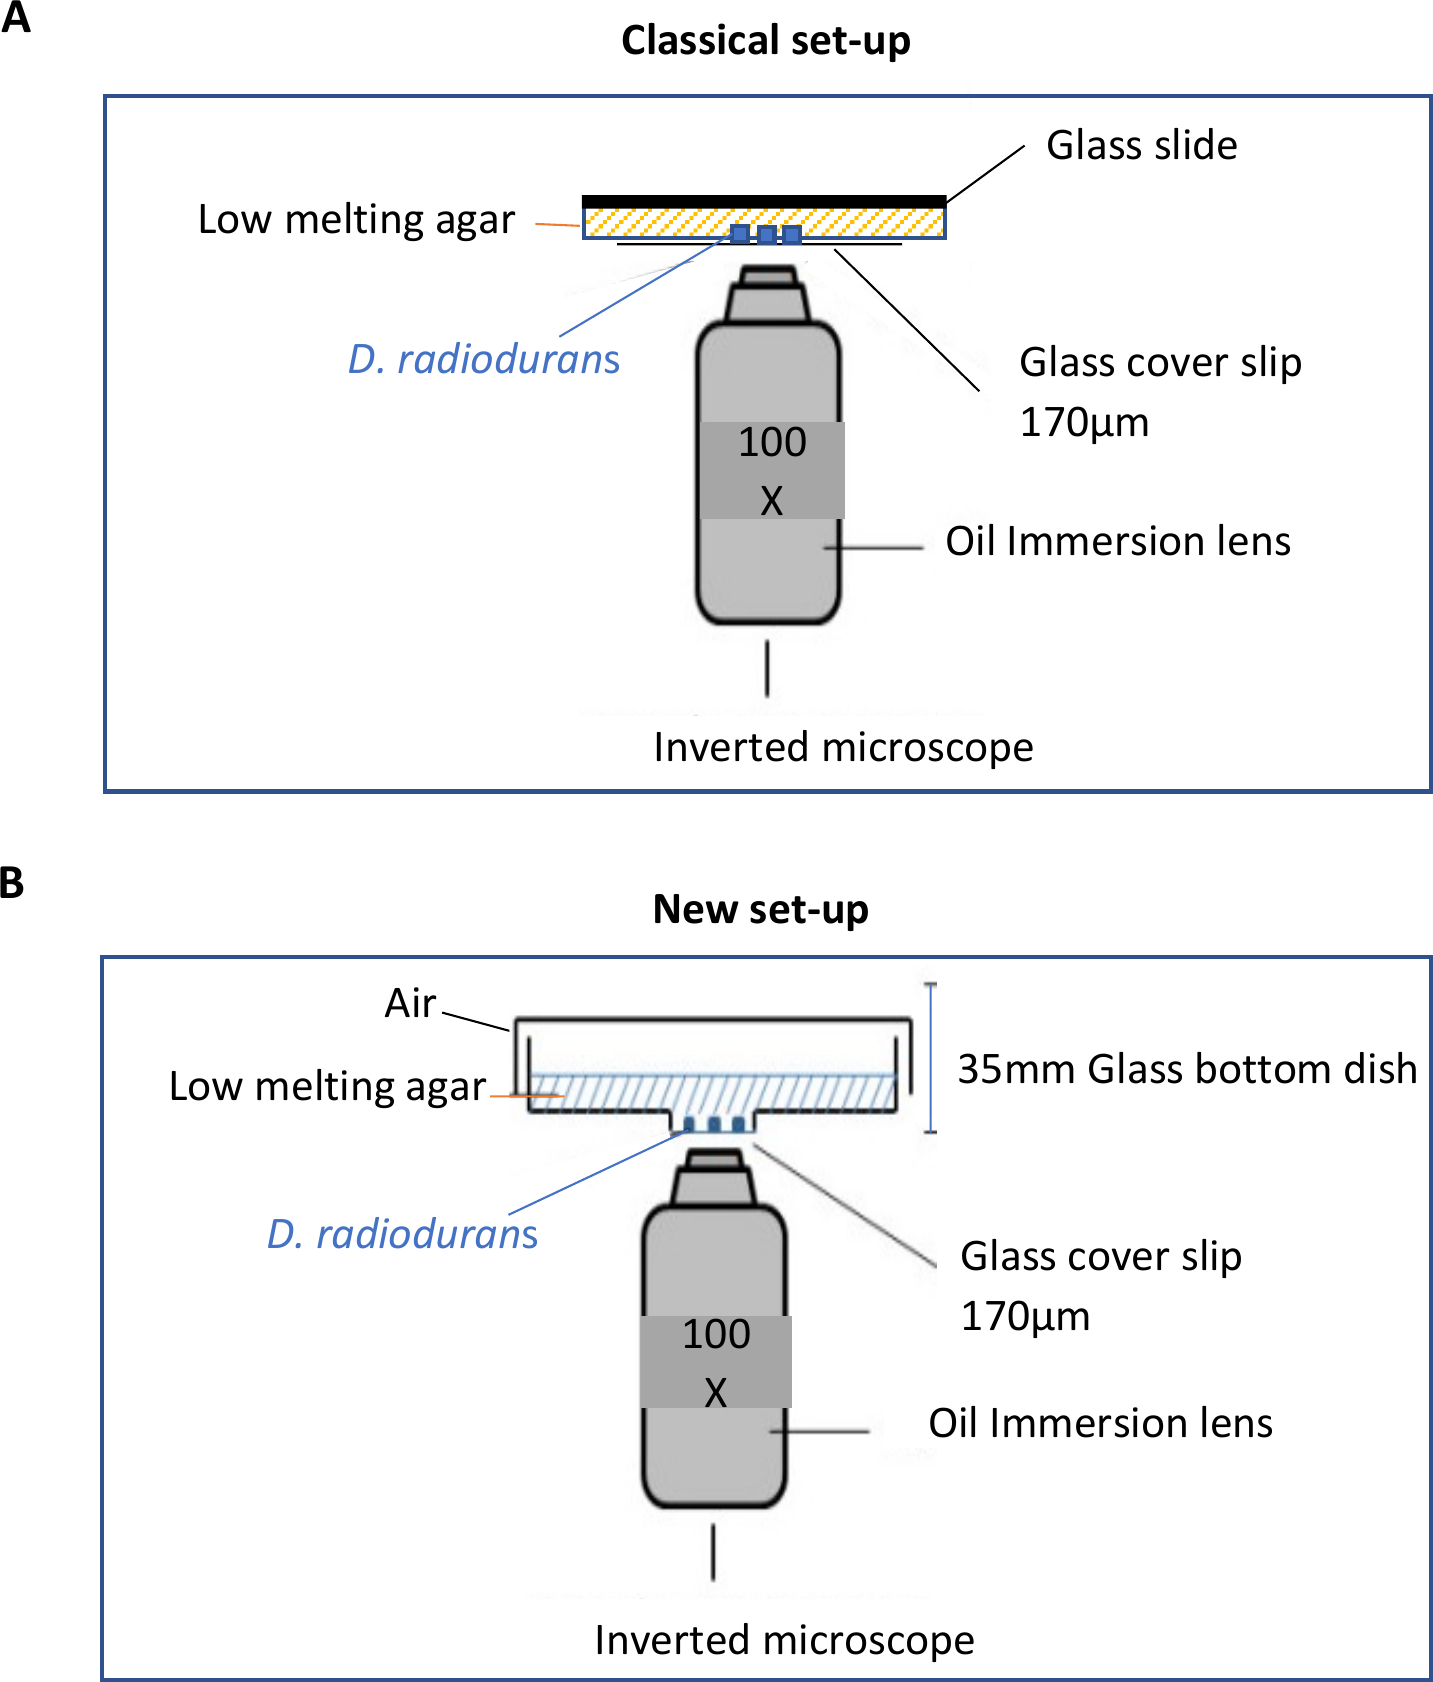
\includegraphics[width=\textwidth]{drad_paper/sfig3.png}
    \titledcaption[Microscopy set-ups for timelapse 3D confocal video-microscopy]{(A) Classical set-up in which cells are seeded on a low melting agarose pad and then overlaid with a glass coverslip. In this set-up, cells are mostly positioned in the same orientation orthogonal to the two successive division planes. (B) New set-up in which cells are deposited on the glass of a glass-bottomed dish and then coated with low melting agarose. The pouring of the melted agarose over the cells results in a wider distribution of cell orientations allowing to view the septation in tilted cells.}
    \label{drad_sfig3}
\end{figure}

\begin{figure}[ht]
    \centering
    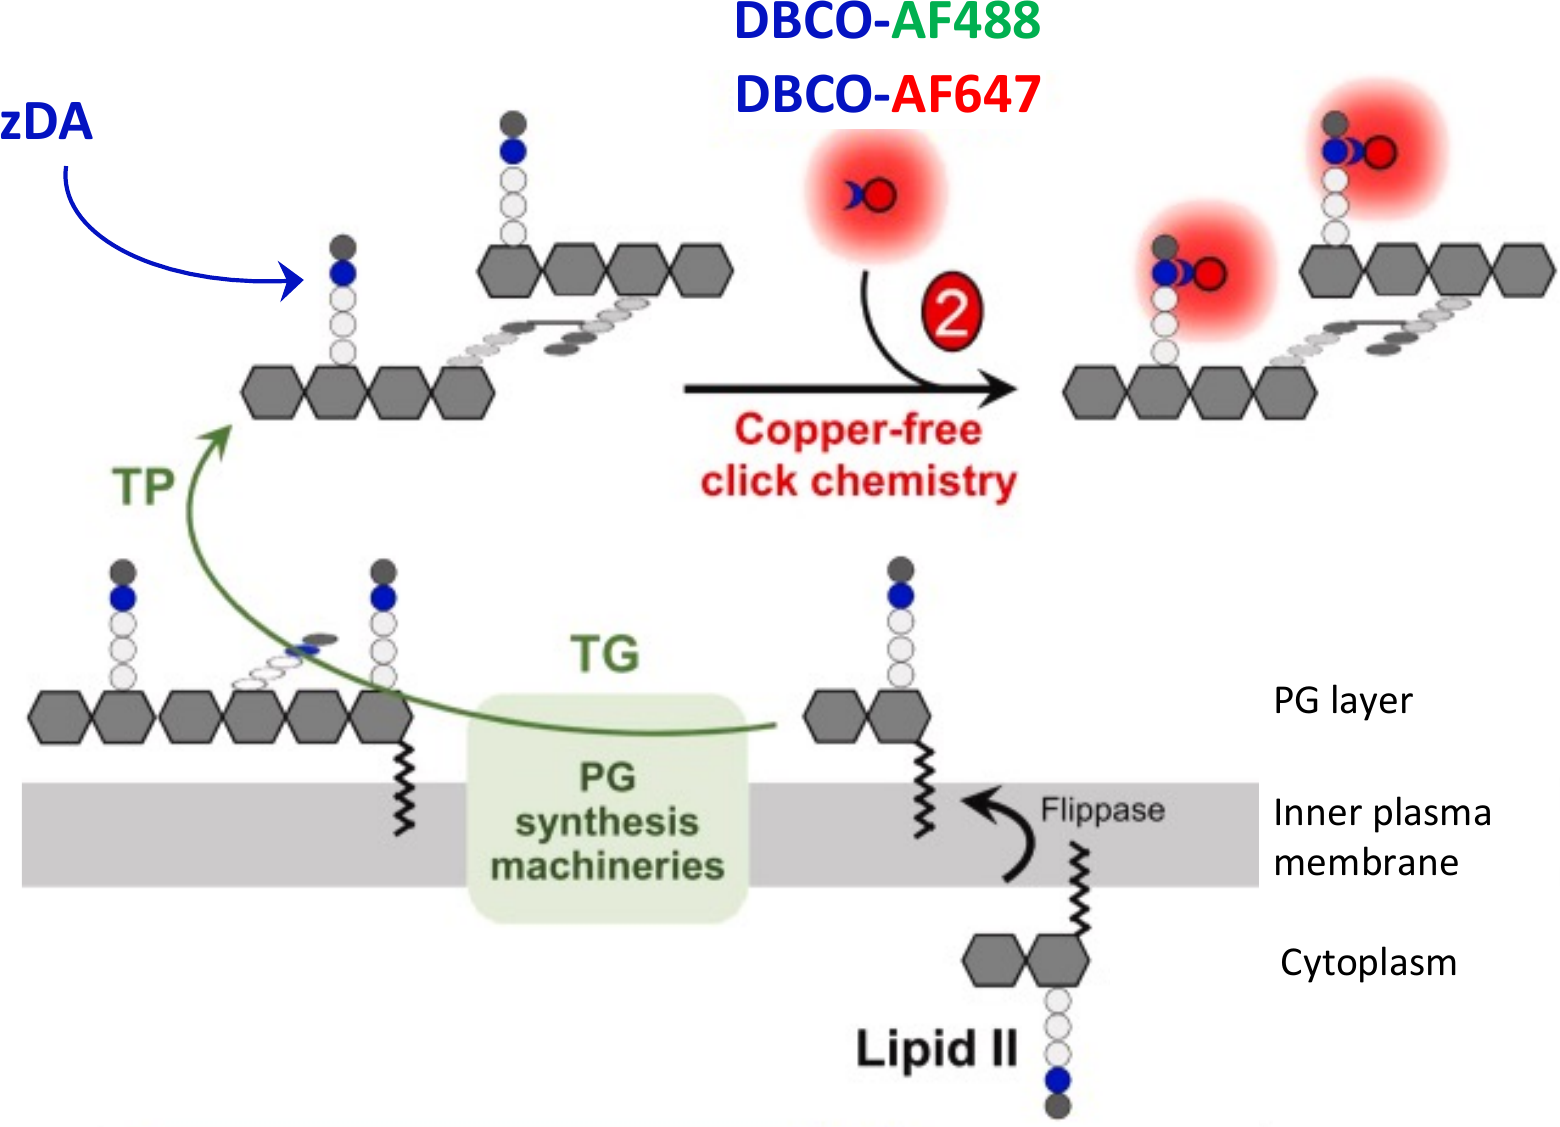
\includegraphics[width=\textwidth]{drad_paper/sfig4.png}
    \titledcaption[PG labelling schematic]{Schematic diagram of the mode of zDA incorporation and labelling of PG in growing D. radiodurans.}
    \label{drad_sfig4}
\end{figure}

\begin{figure}[ht]
    \centering
    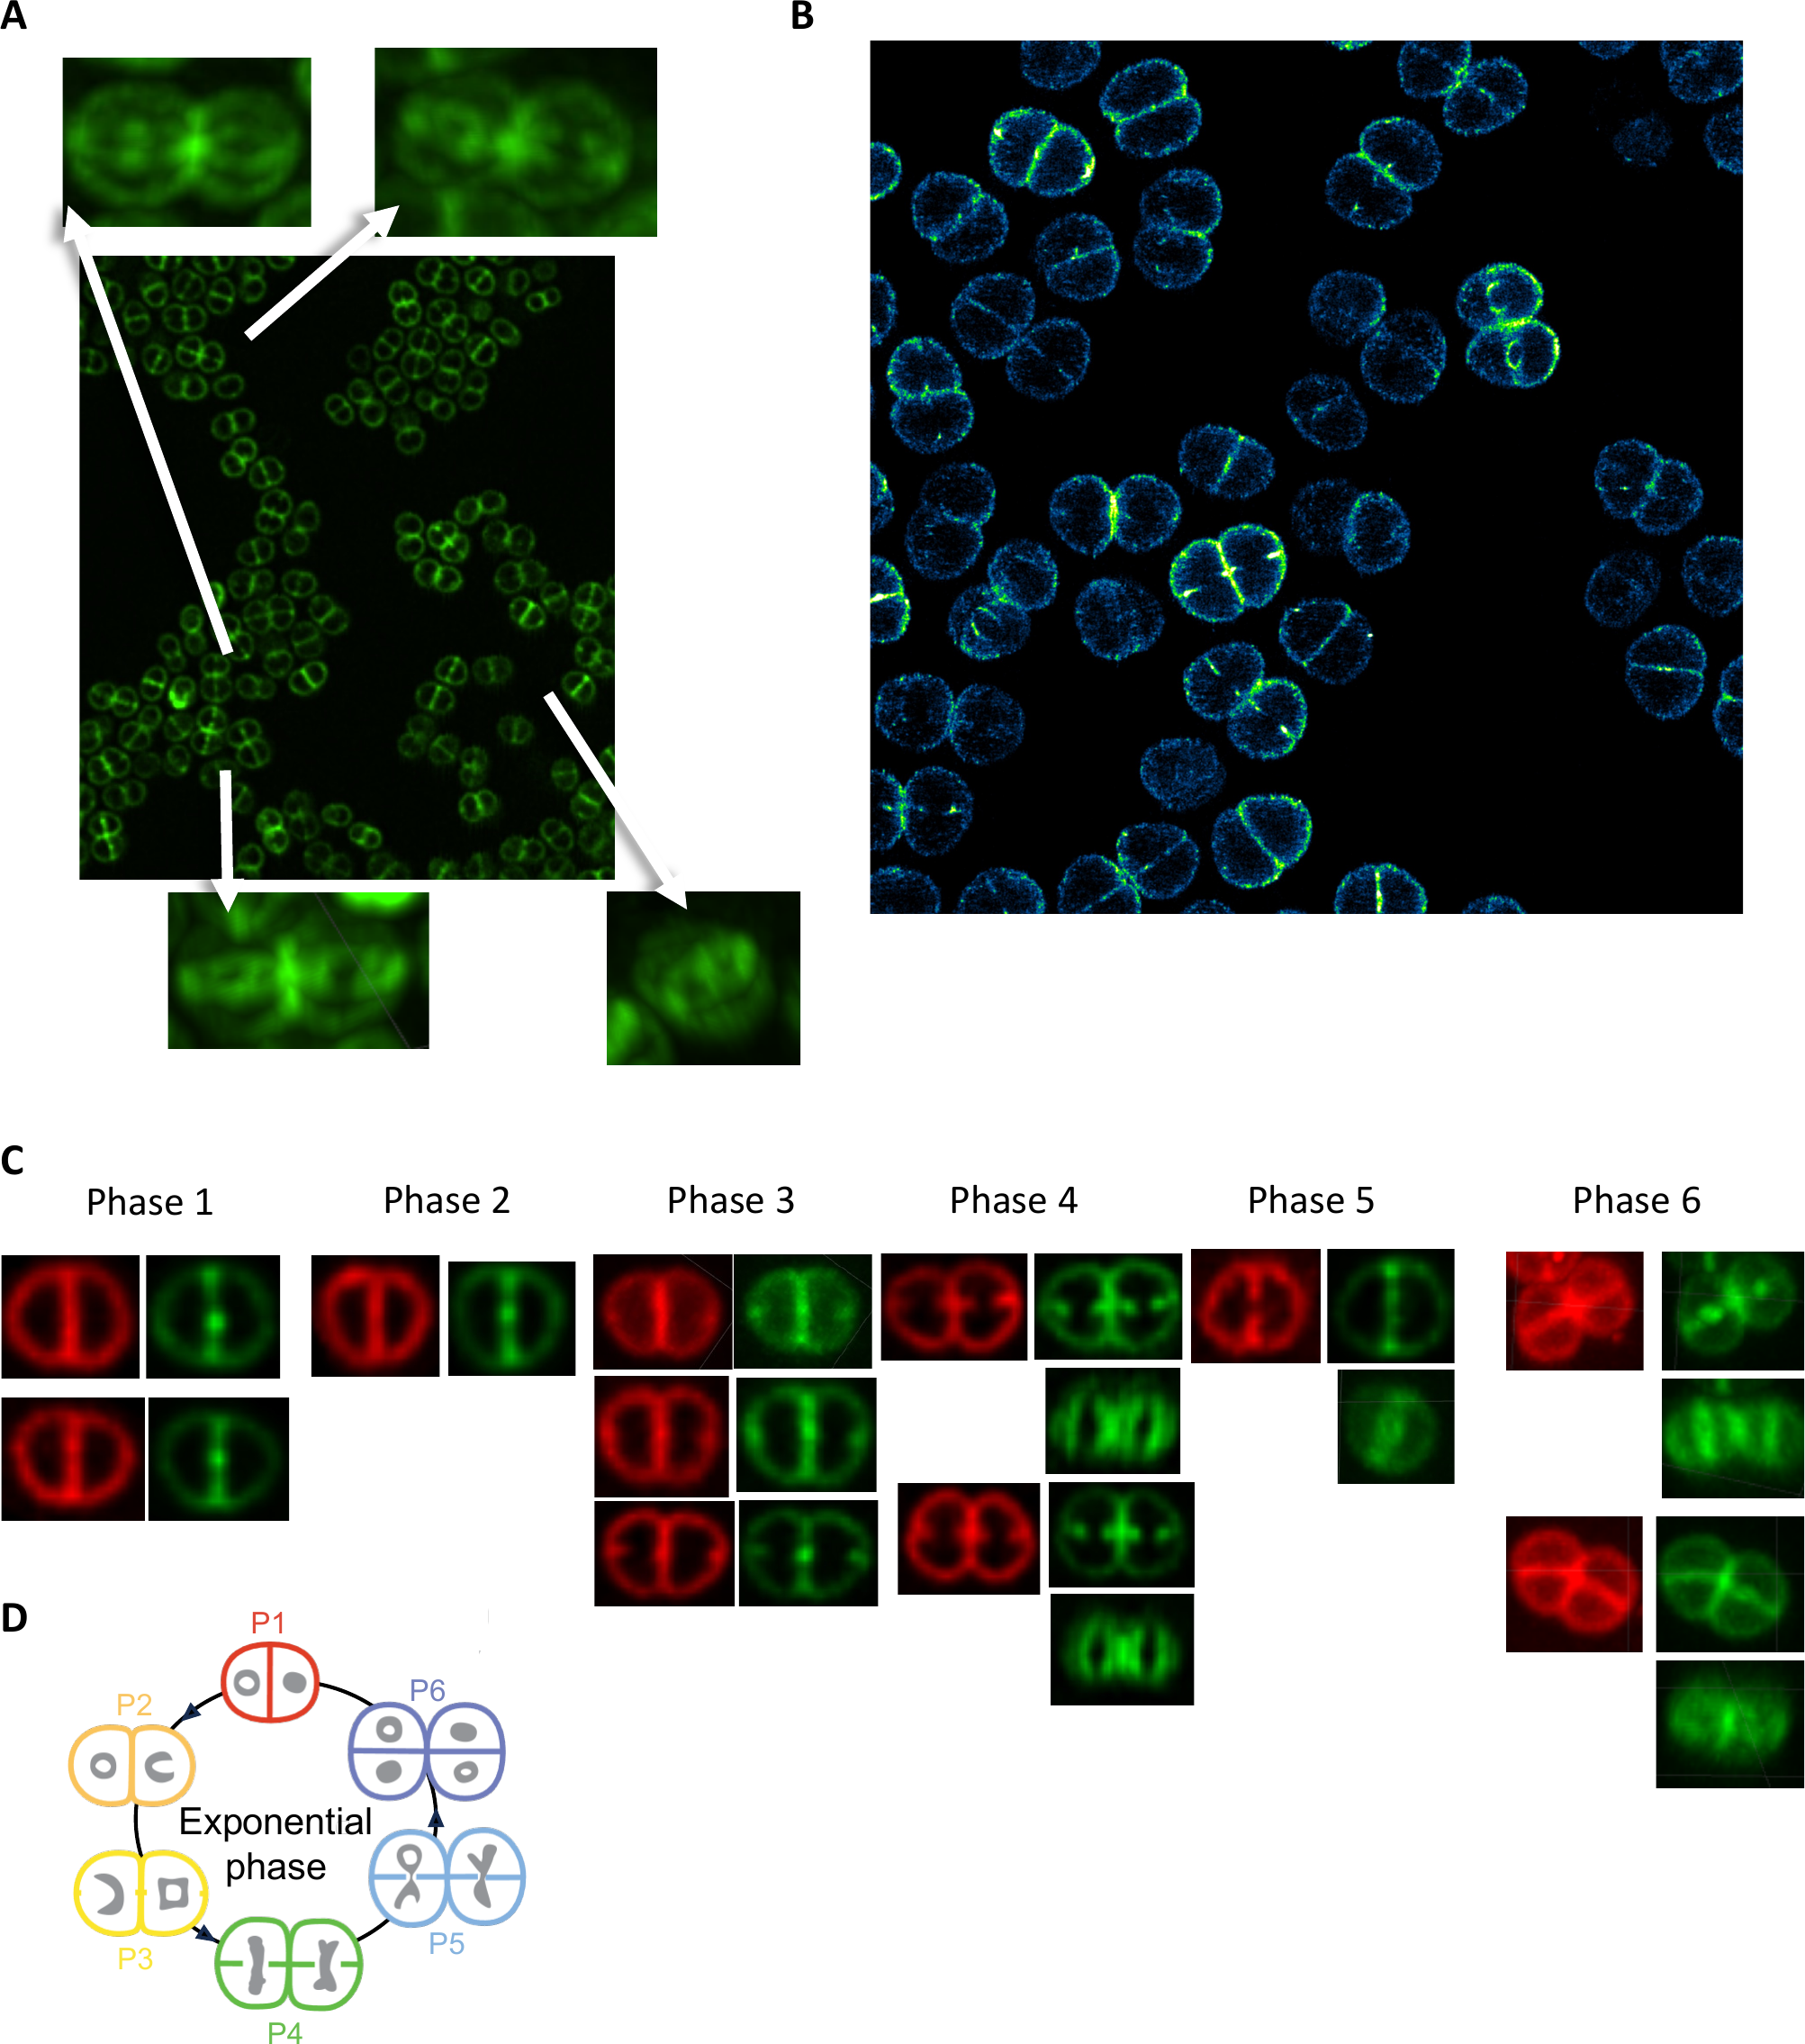
\includegraphics[width=\textwidth]{drad_paper/sfig5.png}
    \titledcaption[PG-labelled D. radiodurans]{Examples of images of PG-labelled growing D. radiodurans viewed by confocal (A) and dSTORM (B) microscopy. (C) Dual labelling of PG (green) and membrane (Nile Red) layers as a function of the phases of the cell cycle. (D) Schematic diagram of the different phases of the D. radiodurans cell cycle starting in phase 1 (P1) as a diad and ending in phase 6 (P6) in the form of a tetrad. The septation process takes place from phases 3 to 6.}
    \label{drad_sfig5}
\end{figure}

\begin{figure}[ht]
    \centering
    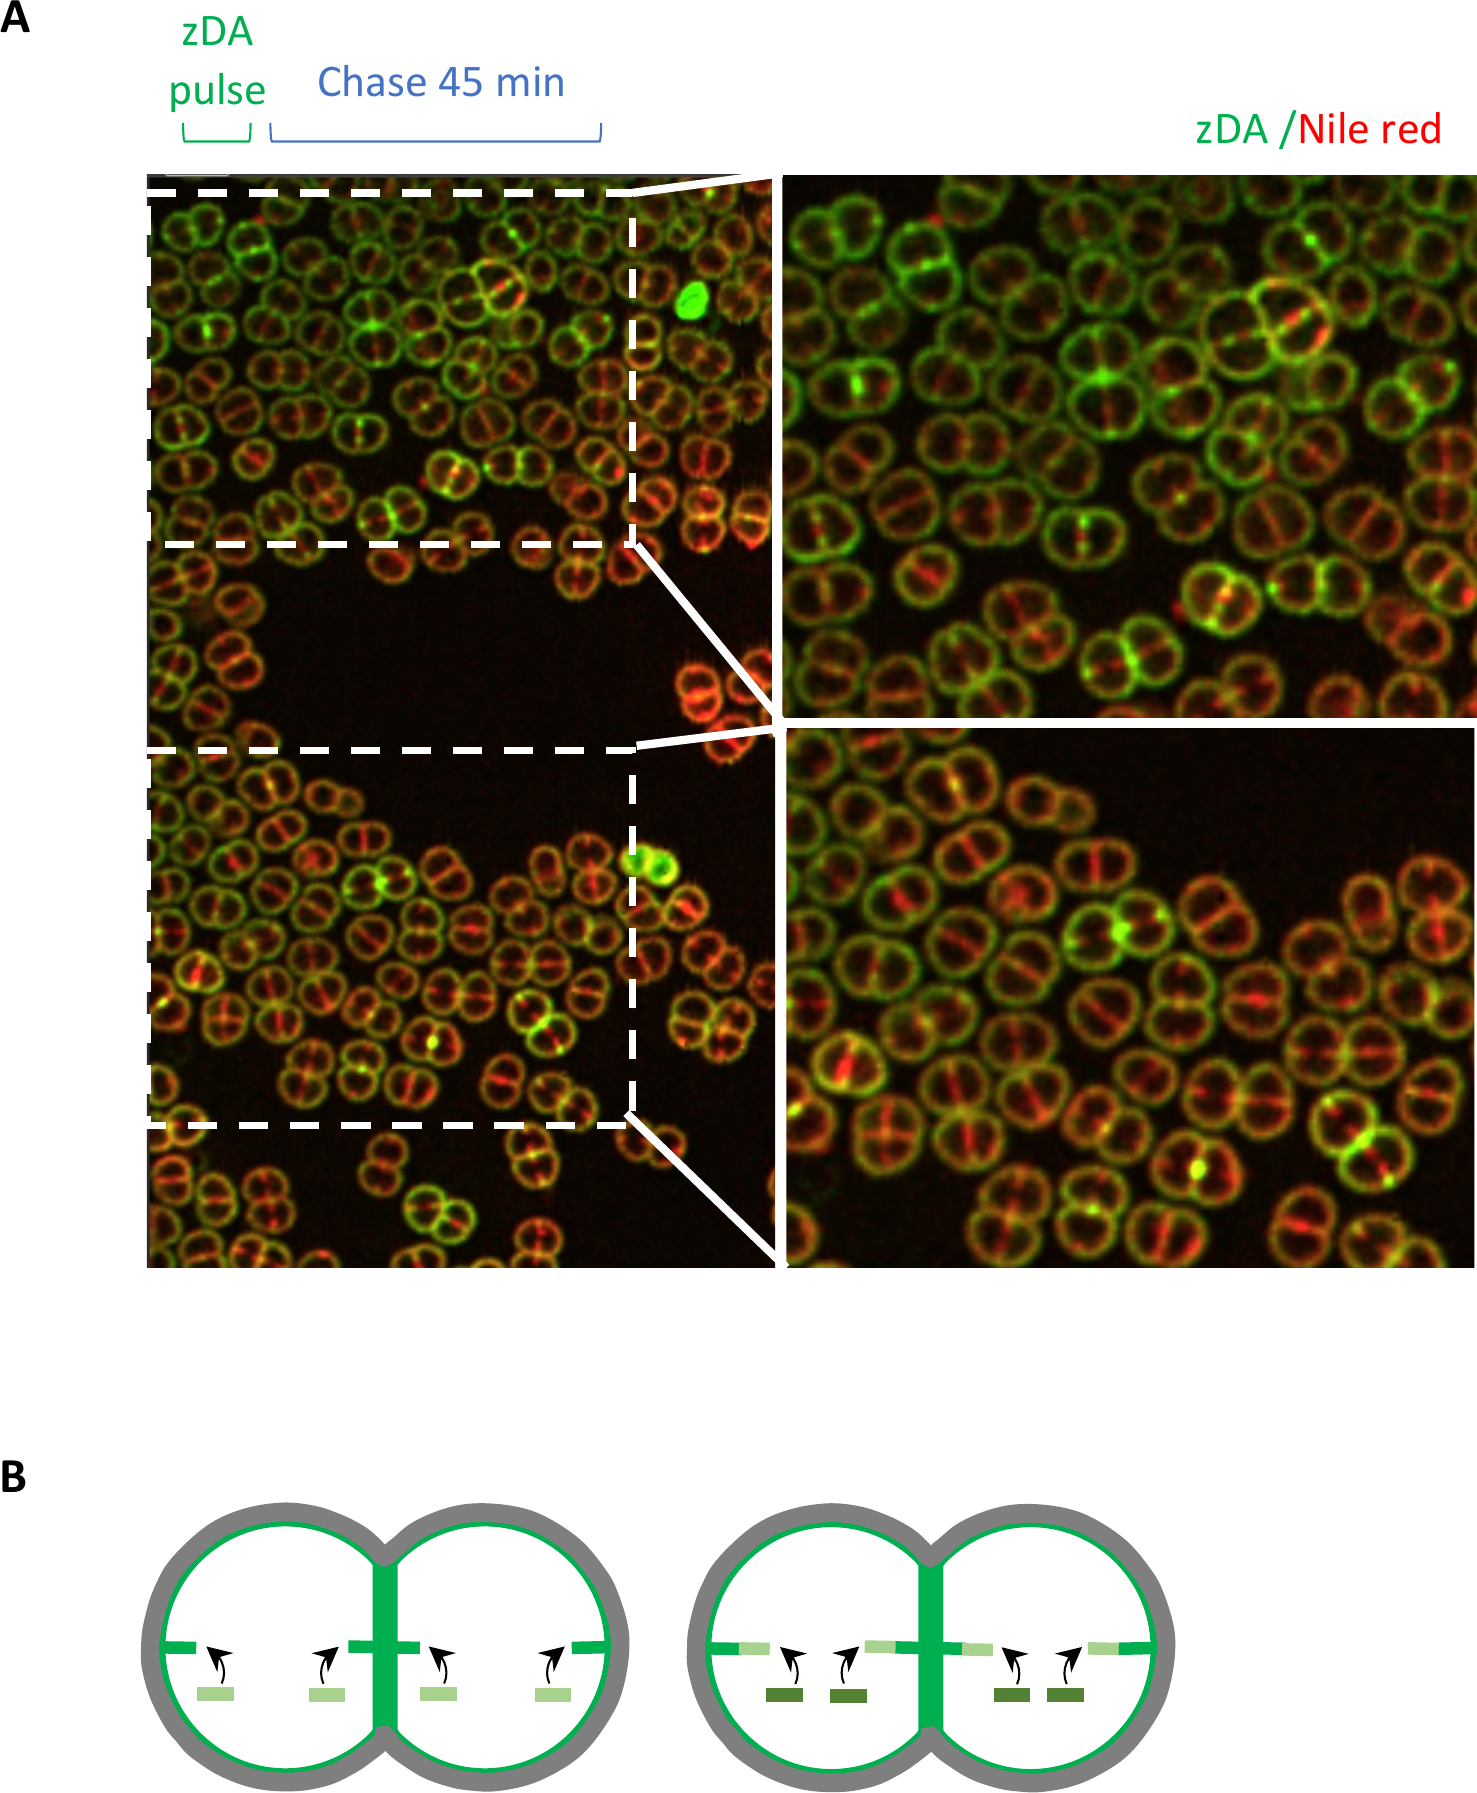
\includegraphics[width=\textwidth]{drad_paper/sfig6.png}
    \titledcaption[Two-color labelled chase experiment]{(A) Examples of two-color confocal microscopy images of PG- and Nile Red-labelled D. radiodurans after a 45 min chase experiment. PG labelling in green and membrane labelling in red. (B) Diagram illustrating the stepwise synthesis of PG at the tip of the growing septa to progressively extend the septa until they are sufficiently close to fuse.}
    \label{drad_sfig6}
\end{figure}

\begin{figure}[ht]
    \centering
    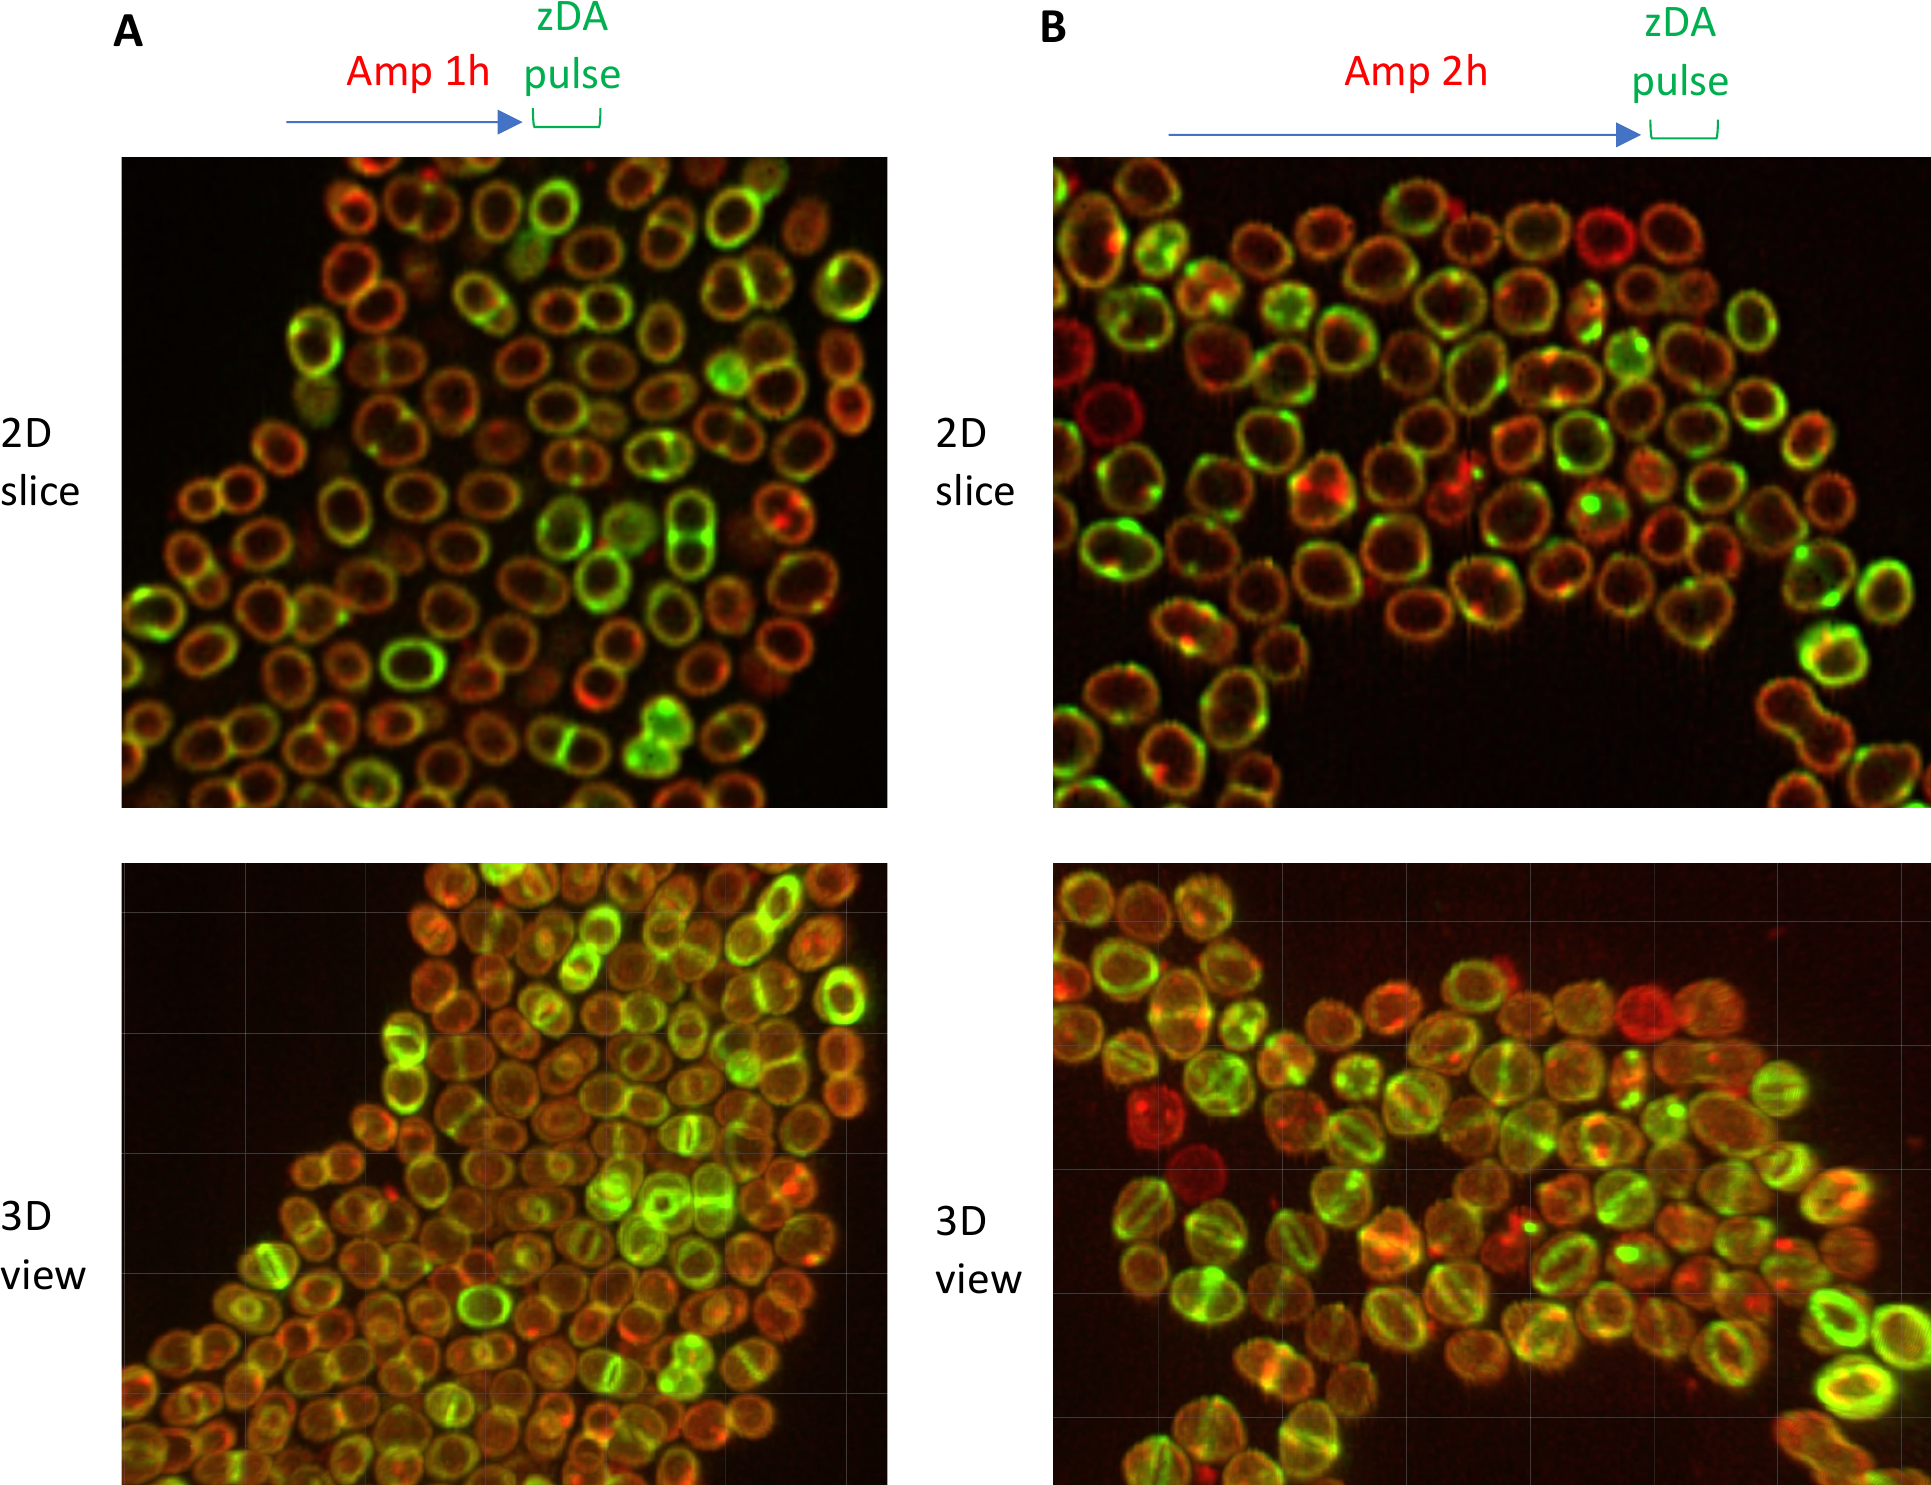
\includegraphics[width=\textwidth]{drad_paper/sfig7.png}
    \titledcaption[Two-color labelled chase experiment with Ampicillin]{Examples of two-color confocal microscopy images of PG- and Nile Red-labelled D. radiodurans after growth in the presence of 1\mu{}g/ml Ampicillin for 1h (A) or 2h (B). PG labelling in green and membrane labelling in red. Top panels: 2D slices through the confocal images. Lower panels: 3D views of the same regions.}
    \label{drad_sfig7}
\end{figure}

\begin{figure}[ht]
    \centering
    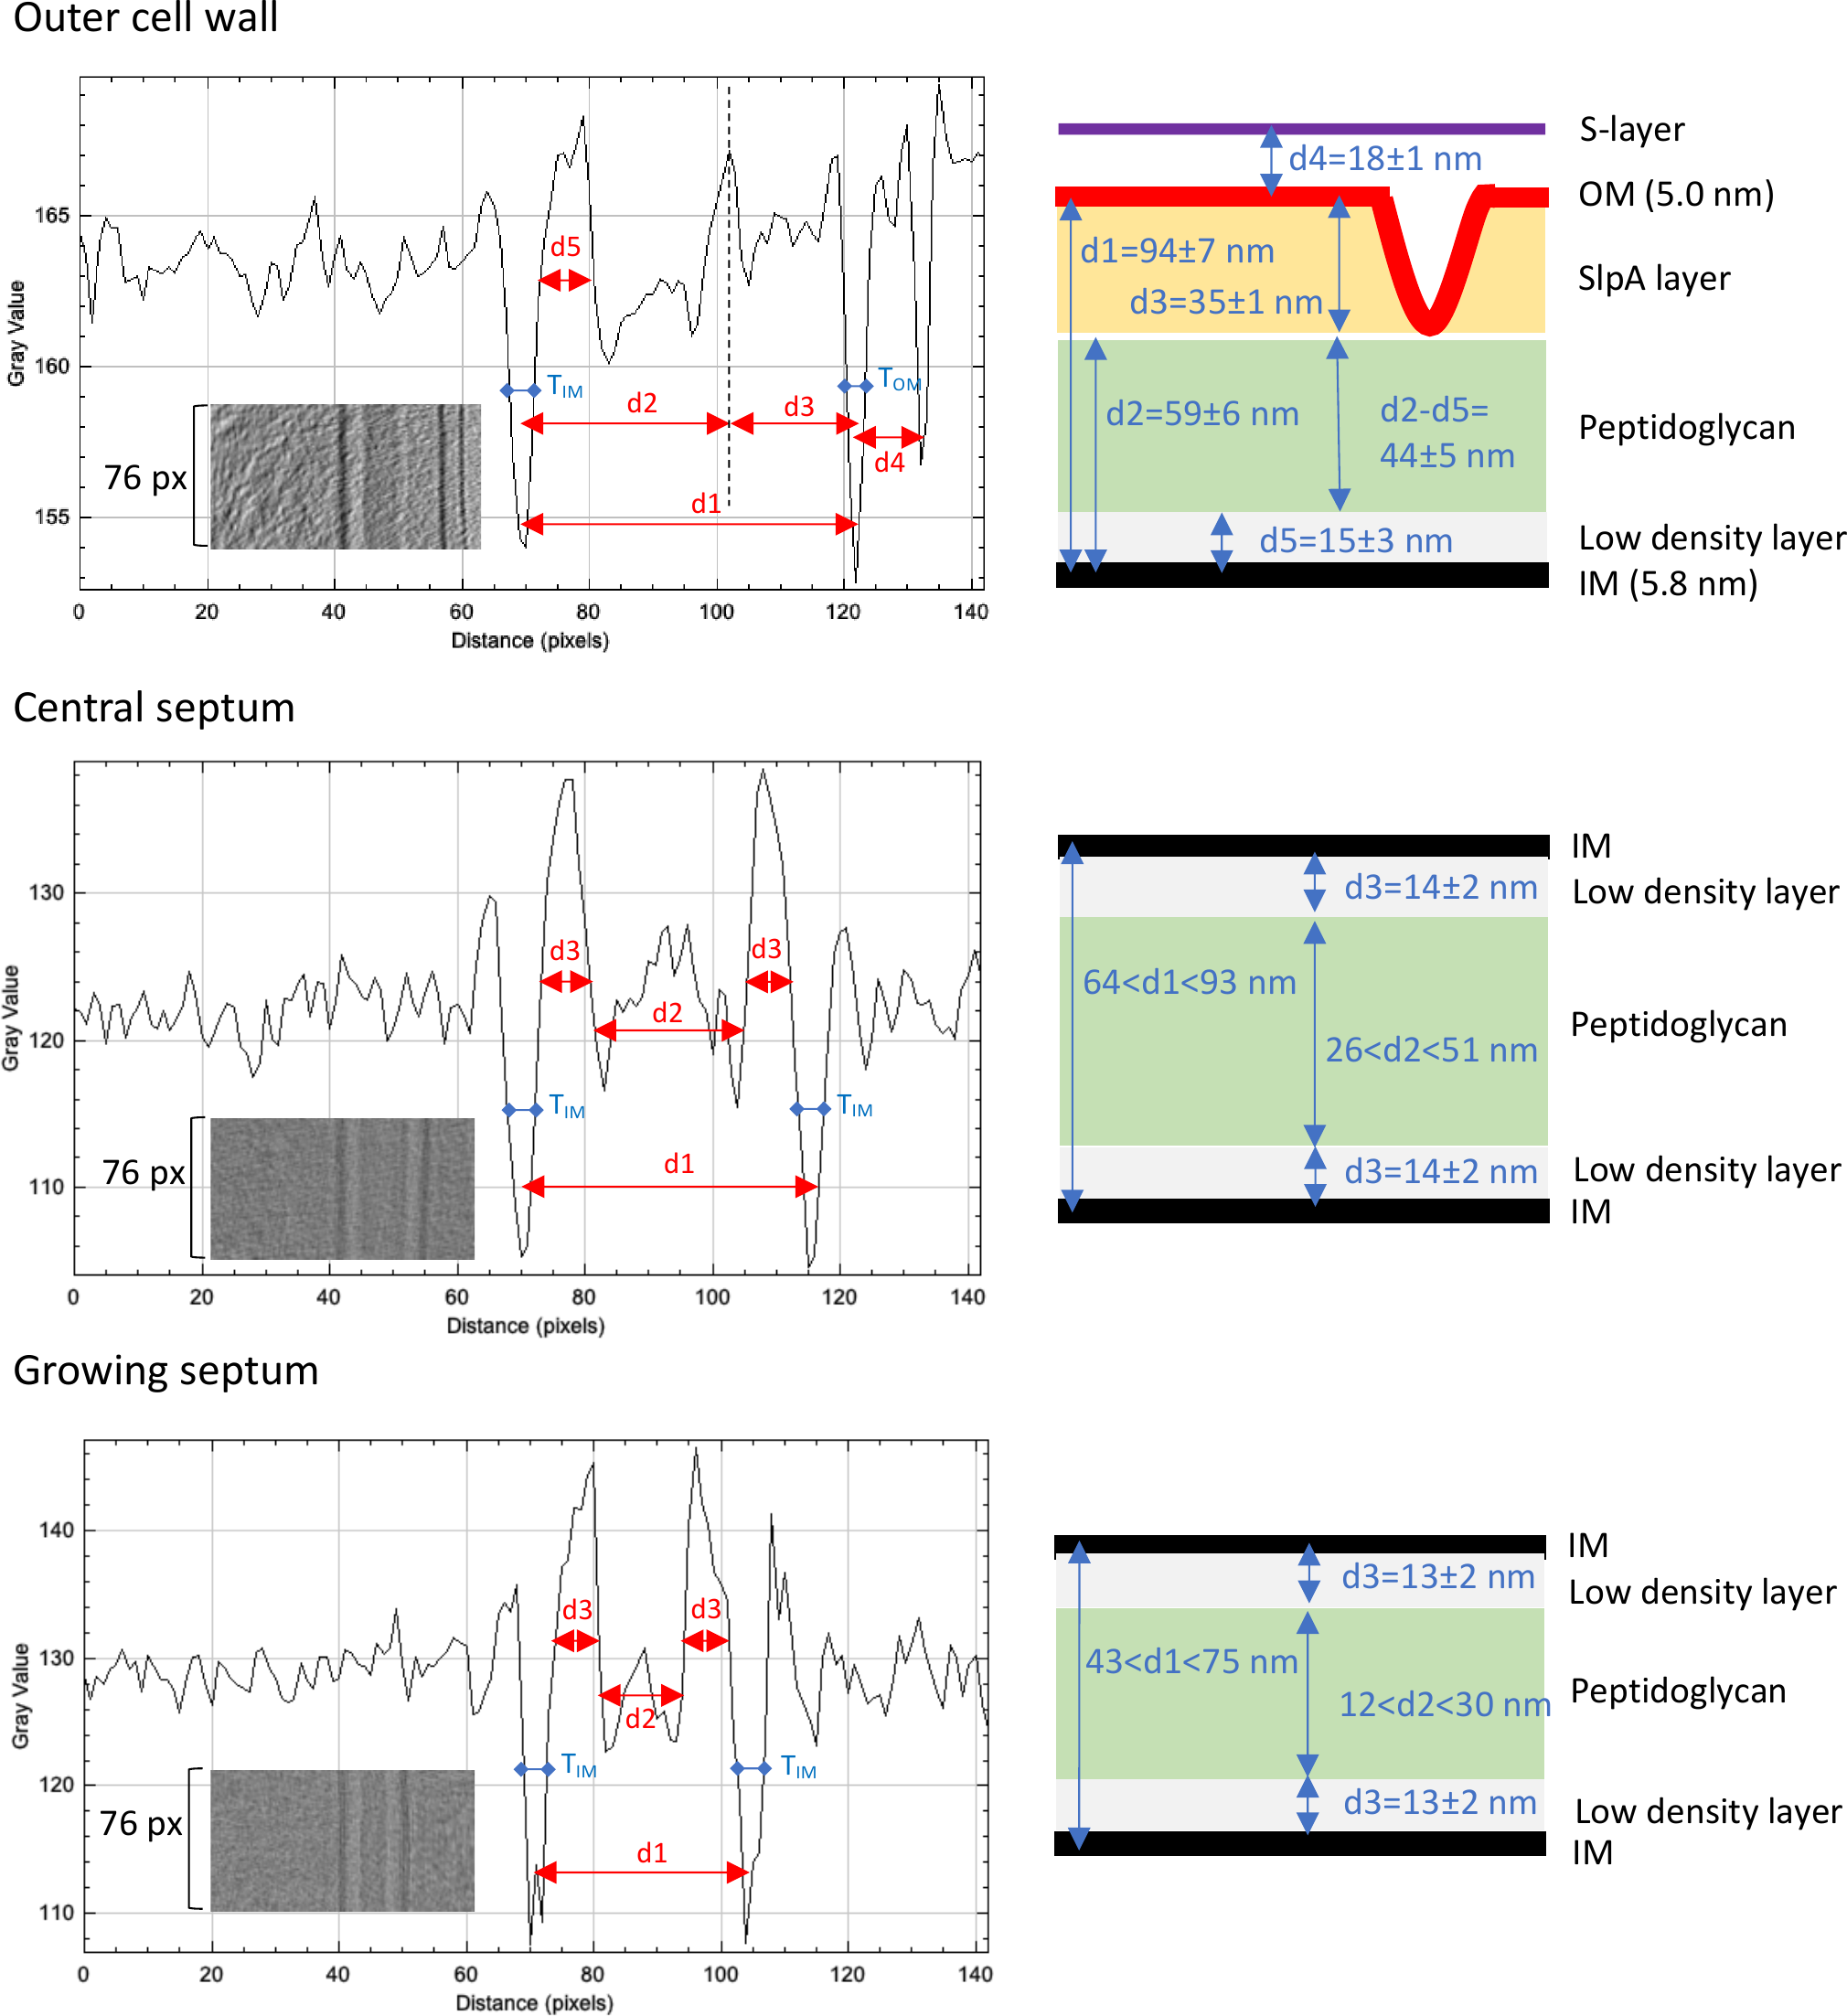
\includegraphics[width=\textwidth]{drad_paper/sfig8.png}
    \titledcaption[1D density profiles of walls and septa]{Typical 1D density profiles obtained for 76-pixel sections of 2D projections of straightened cell walls (illustrated as insets) from the outer cell envelope (top), central septum (middle) and the growing septum (bottom). Various measurements were made to determine the average thicknesses of the different layers composing these distinct cell walls. Distances between the middle of the IM, OM, central white line and the S-layer were measured as shown by the red arrows. Additionally, the thickness of the inner (TIM) and outer (TOM) were measured at mid-peak height as shown with the blue lines. The thickness of the periplasmic space (d5 in top panel and d3/d3' in lower panels) was measured at the base of this positive peak.}
    \label{drad_sfig8}
\end{figure}
